\documentclass[preprint]{elsarticle}

\usepackage{amssymb}
\usepackage{amsmath}
\usepackage{amsfonts}
%\usepackage{cite}
%\usepackage{graphics}
%\usepackage{epsf}
%\usepackage{psfig}
%\usepackage{float}
\usepackage{graphicx}
\usepackage{epstopdf}
%\usepackage[small]{caption2}
%\usepackage{bm}%
%\usepackage{multirow}
%\usepackage{subfigure}
%\usepackage{wrapfig}
%\usepackage{color}
%\usepackage{dsfont}
%\usepackage{amsthm}
%\usepackage{algorithm}
%\usepackage{subfigure}
\usepackage{subcaption}

\graphicspath{{../}}

\DeclareMathOperator*{\argmin}{\arg\!\min}

%\newtheorem{theorem}{Theorem}
%\newtheorem{corollary}[theorem]{Corollary}
%\newtheorem{lemma}[theorem]{Lemma}
%\newtheorem{observation}[theorem]{Observation}
%\newtheorem{proposition}[theorem]{Proposition}
%\newtheorem{definition}[theorem]{Definition}
%\newtheorem{claim}[theorem]{Claim}
%\newtheorem{fact}[theorem]{Fact}
%\newtheorem{assumption}[theorem]{Assumption}
%%\newtheorem{example}[theorem]{Example}
% \newtheorem{remark}[theorem]{Remark}

%\journal{Computers \& Chemical Engineering}
\journal{Applied and Computational Harmonic Analysis Letter}

\begin{document}

\begin{frontmatter}

\title{Parsimonious Representation of Nonlinear Dynamical Systems using Diffusion Maps: A Chemotaxis Case Study}

\author[princeton]{Carmeline~J.~Dsilva\corref{cor1}}
\ead{cdsilva@princeton.edu}
%
\author[technion]{Ronen~Talmon}
\ead{ ronen@ee.technion.ac.il}
%
\author[yale]{Ronald R. Coifman}
\ead{coifman@math.yale.edu}
%
\author[princeton, princetonpacm]{Ioannis~G.~Kevrekidis \corref{cor1}}
\ead{yannis@princeton.edu}
%
\address[princeton]{Department of Chemical and Biological Engineering, Princeton University, Princeton, NJ, 08540, USA}
\address[technion]{Technion - Israel Institute of Technology, Haifa, 3200003, Israel}
\address[yale]{Department of Mathematics, Yale University, New Haven, CT, 06520, USA}
\address[princetonpacm]{Program in Applied and Computational Mathematics, Princeton University, Princeton, NJ, 08540, USA}
%
\cortext[cor1]{Corresponding author}


\begin{abstract}

TODO
\end{abstract}

%\sloppy

\begin{keyword}
TODO
\end{keyword}

\end{frontmatter}


\section{Introduction}

In recent years, data mining algorithms have proven useful for many disciplines and applications \cite{....}. 
%
In particular, for dynamical systems, data-driven methodologies have been shown to be essential when a simple macroscopic model cannot be written analytically due to the complexity of the system.
%
For simulations, the governing model is often very high-dimensional and the macroscale dynamics are not obvious; for experimental systems, an explicit model is often unknown. 
%
For such cases, data obtained from observations and/or simulations of the dynamical system combined with these methodologies give rise to a low-dimensional description which can not only provide insight into the underlying dynamics, but also serve as a first step in constructing macroscale models which are consistent with the observed microscale behavior. 


%For many engineering applications, it is often advantageous or even essential to effectively parameterize a system's dynamics. 
%TODO: add reasons why, potential applications, etc.
%%
%Often, such a parameterization cannot be obtained analytically, due to the complexity of the system.
%%
%For simulations, the governing model is often very high-dimensional and the macroscale dynamics are not obvious; for experimental systems, an explicit model is often unknown. 
%%
%In such cases, we utilize data obtained from observations and/or simulations of the dynamical system, and turn to data-driven analysis methods to provide an accurate low-dimensional description of this data.
%%
%This low-dimensional description can not only provide insight into the underlying dynamics, but also serve as a first step in constructing macroscale models which are consistent with the observed microscale behavior. 
%

Due to the complexity and range of microscale behaviors possible in dynamical systems, we use manifold learning, a nonlinear data-driven analysis technique, to analyze data.
%
Most manifold learning algorithms \cite{...} construct parameterizations of the data through the spectral analysis of a Laplace operator.
%
The data is then embedded in a new, low-dimensional coordinate system given by the eigenvectors of this operator. 
%
Our hope is that these coordinates, obtained in a data-driven manner, will describe the variables which govern the macroscale dynamical behavior of the system and enable us to introduce a reduced macroscale ab-initio model. 

These algorithms were first applied to synthetic data sets to illustrate their geometric properties and flexibility. 
%
Only recently have they been applied to experimental and simulation data, which was possible due to advances in data representation (observers) and metrics. 
%
From a geometric perspective, not all eigenvectors are guaranteed to parameterize unique directions within the data; some eigenvectors are 	``repeated eigendirections'' which describe the same mode. 
%
Identifying those eigenvectors is critical for obtaining an accurate parameterization of the system which captures the true dimensionality of the macroscale dynamics.  
%
This is a challenging task which is often done manually, and few methods have been proposed to automate the identification of the unique eigendirections. 

In this paper, we propose an algorithm to automatically identify the unique eigendirections using local linear regression.
%
We first demonstrate our algorithm on synthetic examples where we have a closed-form solution for the eigenvectors and eigenvalues of the Laplace operator.  
%
This will allow us to validate our proposed approach.
%
We then consider a complex data set from a stochastic dynamical system which models cellular chemotaxis. 
%
The recent advances in observers and metrics, coupled with the proposed approach for factoring out repeated eigendirections, provide a data analysis pipeline which can successfully analyze data from this simulation.
%
This pipeline will allow us to detect changes in the regime/mode of the system, as well as changes in the underlying dimensionality of the macroscale dynamics.  


%\begin{itemize}
%
%\item
%Data driven analysis methods, and in particular, manifold learning, can do many things (dimensionality reduction, reduction in dynamical systems, etc). 
%
%\item
%Manifold learning constructs parameterization of the data through the spectral analysis of a Laplace operator.
%
%\item
%Initially it was used almost exclusively for toy examples/synthetic data (``these people suck").
%
%\item
%Only recently, has it been applied to real (experimental/simulation) data, and this was possible due to advances in observers (data representation) and metrics (``we are awesome"). 
%
%\item
%However, a major limitation (of spectral methods based on a Laplace operator) is identifying the true principal components.
%
%\item For the example of a square/strip, we know everything analytically, and identifying the ``true'' principal components is a problem/not obvious, and depends both on geometry and density
%
%\item While we can ignore/address nonuniform densities through normalization of the Laplace operator, we still have the problem of repeated eigendirections. 
%
%\item Add text about the meaning of the eigenvectors (obtained in the form of eigenvectors of a Laplace operator), as demonstrated in the chemotaxis example. The main idea is the ability to obtain, in a data driven manner, the "true" parsimonious description of the system, which is certain cases (such as particular regimes/modes of the chemotaxis system) may be significantly different from the typical representation and choice of variables used to describe the system (e.g. in the chemotaxis, it will not necessarily be the two fluxes).  
%
%\item
%In this paper, we propose an algorithm to automatically identify those principal components using locally linear regression.
%
%\item
%All of these considerations (recently developed plus what we propose here) provide a data analysis pipeline. We show that this pipeline can successfully analyze data from a complex stochastic dynamical system originated from the study of cellular dynamics (chemotaxis).
%
%\end{itemize}



\section{Manifold Learning Based on Laplace Operators}

Data from dynamical systems is most often high-dimensional, since it is collected at the microscale.
%
However, the macroscale dynamics often evolve to a low-dimensional description. 
%
In such cases, the high-dimensional microscale data will be restricted to a low-dimensional manifold embedded in the high-dimensional space. 
%
Extracting a parameterization of this manifold corresponds to parameterizing the low-dimensional, macroscale dynamics \cite{...}.

Let $z(1), \dots, z(m) \in \mathbb{R}^n$ denote $m$ observations sampled from the dynamical system. 
%
We assume the $n$-dimensional observations $z(i)$ lie on a $d$-dimensional manifold $\mathcal{M}_d$, where $d < n$. 
%
We will show how to extract a $d$-dimensional parameterization of the observations which is consistent with the geometry of the manifold. 

\subsection{Eigenfunctions of the Laplace-Beltrami operator}

\begin{figure}[t]
\centering
\begin{subfigure}{0.45\textwidth}
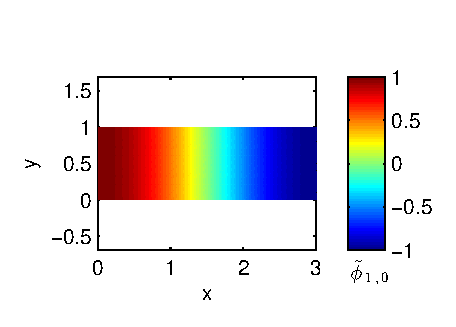
\includegraphics[width=\textwidth]{strip_cnts1}
\caption{}
\end{subfigure}
%
\begin{subfigure}{0.45\textwidth}
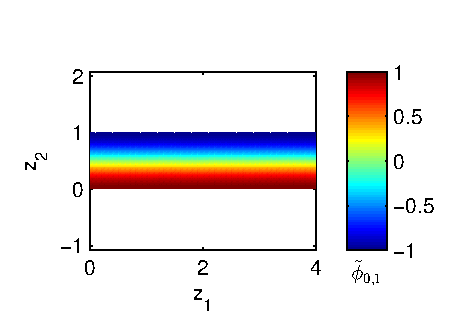
\includegraphics[width=\textwidth]{strip_cnts2}
\caption{}
\end{subfigure}
\caption{Two-dimensional strip colored by the eigenfunction (a) $\tilde{\phi}_{1, 0} = \cos \left( \frac{\pi z_1}{L_1} \right)$, and (b) $\tilde{\phi}_{0, 1} = \cos \left( \frac{\pi z_2}{L_2} \right)$ .}
\label{fig:strip_efuncs}
\end{figure}


We start by considering a continuous setting where rigorous analysis is available for specific examples. 
%
In such an example, we will show that the existence of repeated eigendirections is inherent to the manifold learning setup based on Laplace operators, and that the identification of the unique eigendirections is nontrivial. 
%
The existence of these challenges in the continuous setting implies that, even in the limit of infinite data, such repeated eigendirections still pose a problem for analysis. 
%
Thus, we consider the problem of parameterizing a continuous $d$-dimensional manifold $\mathcal{M}_d$ embedded in $\mathbb{R}^n$.
%
For linear hyperplanes, the principal axes parameterize the manifold.
%
However, in the case when the manifold is nonlinear, the set of coordinates is not readily apparent. 

In recent years, the eigenfunctions of the Laplace-Beltrami operator have been used to parameterize the manifold \cite{Belkin2003, coifman2005geometric, singer2008non}. 
%
To illustrate why these eigenfunctions provide appropriate coordinates, consider a two-dimensional strip with edge lengths $L_1$ and $L_2$. 
%
The eigenvalues of the Laplace-Beltrami operator with Neumann boundary conditions are given by
\begin{equation} \label{eq:evals}
\tilde{\mu}_{k_1, k_2} = \left( \frac{k_1 \pi}{L_1} \right)^2 + \left( \frac{k_2 \pi}{L_2} \right)^2
\end{equation}
for $k_1, k_2 = 0, 1, 2, \dots$,
and the corresponding eigenfunctions are 
\begin{equation} \label{eq:efuncs}
\tilde{\phi}_{k_1, k_2} = \cos \left( \frac{k_1 \pi z_1}{L_1} \right) \cos \left( \frac{k_2 \pi z_2}{L_2} \right)
\end{equation}
where $z_1$ and $z_2$ denote the two coordinates of the strip \cite{singer2008non}. 
%
We note that the eigenfunctions $\tilde{\phi}_{1, 0} = \cos \left( \frac{\pi z_1}{L_1} \right)$ and $\tilde{\phi}_{0, 1} = \cos \left( \frac{\pi z_2}{L_2} \right)$ are one-to-one with the $z_1$ and $z_2$ coordinates, respectively, and therefore yield a parameterization of the underlying manifold (see Figure~\ref{fig:strip_efuncs}). 
%
Furthermore, the corresponding eigenvalues $\tilde{\mu}_{1,0}$ and $\tilde{\mu}_{0,1}$ provide a measure of $L_1$ versus $L_2$: as the ratio between $L_1$ and $L_2$ increases, the gap between $\tilde{\mu}_{1,0}$ and $\tilde{\mu}_{0,1}$ also increases (this will be discussed further in Section~\ref{sec:relative_lengths}).
%
The analytic form of the eigenfunctions in \eqref{eq:efuncs} illustrates the two issues we address in this paper. 
%
First, $z_1$ and $z_2$ are not necessarily decoupled in subsequent eigenfunctions. 
TODO: address this in later section
%
Second, eigenfunctions with $k_1+k_2 \ge 2$ do not describe any additional directions along the strip; we will refer to these as ``repeated eigendirections,'' and we will refer to the eigenfunctions with $k_1+k_2 =1$ as ``unique eigendirections.''
%
We note that, although the eigenfunctions can only be written analytically for very special cases, it has been observed empirically that the eigenfunctions often provide appropriate coordinates to parameterize more complex, nonlinear manifolds. 


\subsection{Discrete approximation of the Laplace-Beltrami operator: diffusion maps}

\begin{figure}[t]
\centering
\begin{subfigure}{0.45\textwidth}
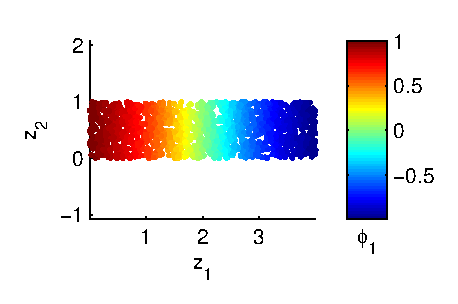
\includegraphics[width=\textwidth]{strip_discrete1}
\caption{}
\end{subfigure}
%
\begin{subfigure}{0.45\textwidth}
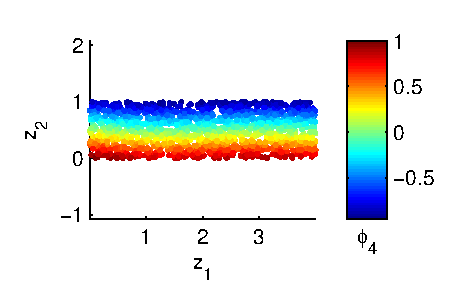
\includegraphics[width=\textwidth]{strip_discrete4}
\caption{}
\end{subfigure}

\begin{subfigure}{0.45\textwidth}
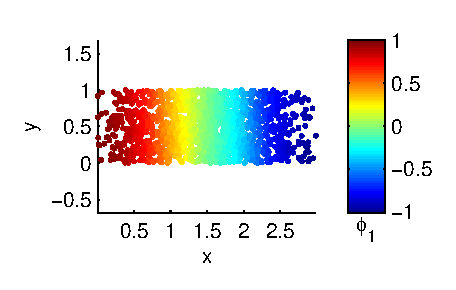
\includegraphics[width=\textwidth]{strip_nonuniform1}
\caption{}
\end{subfigure}
%
\begin{subfigure}{0.45\textwidth}
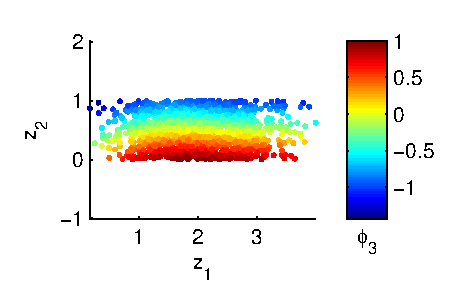
\includegraphics[width=\textwidth]{strip_nonuniform2}
\caption{}
\end{subfigure}
\caption{(a, b) Two-dimensional strip with uniform sampling colored by the (a) first, and (b) fourth (non-trivial) eigenvector from diffusion maps. (c, d) Two-dimensional strip with data sampled from a Gaussian distribution in $z_1$ and sampled uniformly in $z_2$, colored by the (c) first, and (d) third (non-trivial) eigenvector from diffusion maps. Note that in both cases we uncover parameterizations which are one-to-one with $z_1$ and $z_2$. }
\label{fig:strip_evecs}
\end{figure}

In most applications, we are not given a description of the continuous manifold. 
%
Instead, we are given data {\em sampled} from the underlying manifold, and we would like to uncover a parameterization of the data.
%
We will do this by constructing a matrix which approximates the Laplace-Beltrami operator. 
%
It was shown in \cite{...} that, in the limit of infinite data, the discrete Laplacian constructed from data converges pointwise to the continuous Laplace-Beltrami operator on the manifold. 
%
As a result, the eigenvectors of the discrete Laplacian approximate the eigenfunctions of this continuous operator \cite{...}.

Given observations $z(1), \dots, z(m) \in \mathcal{M}_d$, we construct the matrix $W \in \mathbb{R}^{m \times m}$, with
\begin{equation} \label{eq:W}
W_{ij} = \exp \left( -\frac{\|z(i) - z(j) \|^2}{\epsilon^2} \right), \ i,j=1,\ldots,m,
\end{equation}
where $\| \cdot \|$ denotes the appropriate norm for the observations, and $\epsilon$ is a characteristic distance between the observations. 
%
The kernel's scale $\epsilon$ can be chosen using several heuristics \cite{coifman2008graph, rohrdanz2011determination}; we often take $\epsilon$ to be the median of the pairwise distances between the data points.
%
We then construct the diagonal matrix $D \in \mathbb{R}^{m \times m}$, with $D_{ii} = \sum_j W_{ij}$, and the matrix $A  = D^{-1} W.$
%
In the limit of infinite data uniformly sampled from $\mathcal{M}_d$ ($m \rightarrow \infty$ and $\epsilon \rightarrow 0$ with the appropriate rate), the matrix $I-A$ approaches the Laplace-Beltrami operator on the manifold $\mathcal{M}_d$ \cite{coifman2006geometric}. 
%
Therefore, the eigenvectors $\phi_0, \phi_1, \dots, \phi_{m-1}$ of $A$ approximate the eigenfunctions of the Laplace-Beltrami operator on $\mathcal{M}_d$,
and the eigenvalues $\mu_0, \mu_1, \dots, \mu_{m-1}$ of $A$ are related to the eigenvalues of the continuous operator by 
\begin{equation} \label{eq:evals_relationship}
\mu_k = \exp \left( -\frac{\epsilon^2}{4} \tilde{\mu}_{k_1, k_2}  \right).
\end{equation}
%

However, the data need not be sampled uniformly from the underlying manifold.
%
If the data $z(1), \dots, z(m)$ are sampled from $\mathcal{M}_d$ with some density $q$, then the matrix $I-A$ approximates the Fokker-Planck operator, 
\begin{equation}
(I-A) \phi \rightarrow \nabla^2 \phi - \nabla U \cdot \nabla \phi, 
\end{equation}
where $U = -2 \log q$. 
%
Alternatively, one can factor out the density effects in the diffusion maps matrix.
%
Given data $z(1), \dots, z(m) \in \mathcal{M}_d$, we construct the matrix
%
\begin{equation}
\tilde{W} = D^{-1} W D^{-1}.
\end{equation}
%
Pre- and post-multiplication by $D^{-1}$ removes any density effects from $W$. 
%
We then construct the diagonal matrix $\tilde{D} \in \mathbb{R}^{m \times m}$, with $\tilde{D}_{ii} = \sum_j \tilde{W}_{ij}$, and the matrix $\tilde{A}  = \tilde{D}^{-1} \tilde{W}.$
%
The matrix $\tilde{A}$ is comparable to the matrix $A$, but with sampling density effects removed, such that $I-\tilde{A}$ approaches the Laplace-Beltrami operator even if the data is nonuniformly sampled from the underlying manifold \cite{coifman2005geometric}. 

As discussed previously, the eigenfunctions provide a parameterization of the manifold, such that $\phi_{j}(i)$ yields the $j^{th}$ embedding coordinate for $z(i)$; this embedding is called diffusion maps \cite{...}.
%
We order the eigenvectors such that $|\mu_0| \ge |\mu_1| \ge \dots \ge |\mu_{m-1}|$.%, and if the data do lie on a low-dimensional manifold, we only need to retain a few of the leading eigenvectors to adequately describe the data.
%
Because the matrix $A$ is row-stochastic ($\sum_j A_{ij} = 1$),  $\mu_0 = 1$ and $\phi_0$ is a trivial constant vector.

Figure~\ref{fig:strip_evecs} shows data sampled from a strip, colored by diffusion maps eigenvectors. 
%
In cases of both uniform and nonuniform sampling, the eigenvectors are one-to-one with $z_1$ and $z_2$, and thus parameterize the manifold. 
%
Although we have considered a very simple example for illustrative purposes, common practice is to use these tools for high-dimensional, nonlinear data sets.

From the previous section, we know that the eigenfunctions with $(k_1, k_2) =(1, 0)$ and $(k_1, k_2) =(0, 1)$ provide embedding coordinates for the manifold; these two eigenfunctions are both uncoupled and not repeated.  
%
From \eqref{eq:evals}, we see that if we sort the eigenvectors by the magnitude of the corresponding eigenvalues, these eigenvectors are guaranteed to appear before any coupled or repeated eigendirections. 
%
However, these two eigenvectors are {\em not} guaranteed to appear as the first two (non-trivial) eigenvectors, as harmonics of the first eigendirection (i.e., $\cos \left( n \pi z_1 / L_1 \right)$ with $n > 1$) could appear before the second.
%
In practice, identifying which eigenvectors correspond to unique eigendirections is nontrivial, as the correspondence between the original data and the coordinates which parameterize the manifold are unknown.
%
We note that, in contrast to our simple illustrative example, for most data sets of interest, the coordinates for the underlying manifold cannot easily be obtained from the coordinates of the original data. 

\section{Identifying the Informative Eigenvectors }

Common practice is to order the eigenvectors by the magnitude of the corresponding eigenvalues, assuming that the leading eigenvectors provide a parameterization of the underlying manifold.
%
However, as discussed in the previous section, some eigenvectors are higher harmonics of previous eigenvectors and do not describe new directions in the data set \cite{gerber2007robust}.
%
For the case where $\mathcal{M}_d$ is a $2$-dimensional strip with edge lengths $L_1  > L_2$,
recall that the eigenfunctions $\tilde{\phi}_{1,0} = \cos \left(  {\pi z_1}/{L_1} \right)$ and  $\tilde{\phi}_{0,1} = \cos \left(  {\pi z_2}/{L_2} \right)$ provide embedding coordinates for the manifold $\mathcal{M}_d$. 
%
However, these two eigenvectors $\tilde{\phi}_{1, 0}$ and $\tilde{\phi}_{0, 1}$ are not guaranteed to correspond to the two smallest (non-trivial) eigenvalues (the largest eigenvalue will always be $\tilde{\mu}_{0,0} = 1$ and correspond to a constant eigenfunction; these eigenvalues are related to the eigenvalues $\mu_k$ of the discrete operator via \eqref{eq:evals_relationship}). 
%
In fact, if $L_1 > 2 L_2$, then $\tilde{\mu}_{2, 0} < \tilde{\mu}_{0, 1}$, and so the second (non-trivial) eigenvector (when the eigenvectors are ordered by their corresponding eigenvalues) will be a repeated eigendirection of the first and still parameterize $z_1$ (see Figure~\ref{fig:strip_harmonics}).
%
We therefore require a methodology to automatically detect which eigenvectors are harmonics of each other. 
%
Utilizing only the eigenvectors $\phi_i$ which correspond to unique eigendirections yields the most parsimonious representation of the data.
%
We will show how we can automatically detect these eigenvectors to obtain a meaningful representation of the data.
%
Furthermore, the corresponding eigenvalues provide us with a measure of the relative lengths of the data set along these unique eigendirections. 


\subsection{Algorithm: local linear regression}

\begin{figure}[t]
\centering
\begin{subfigure}{0.45\textwidth}
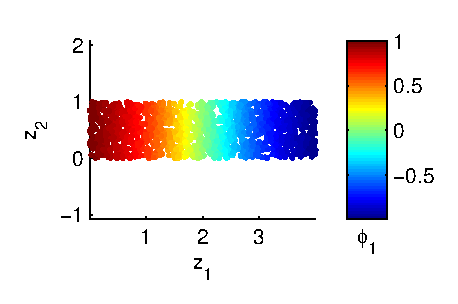
\includegraphics[width=\textwidth]{strip_discrete1}
\end{subfigure}
%
\begin{subfigure}{0.45\textwidth}
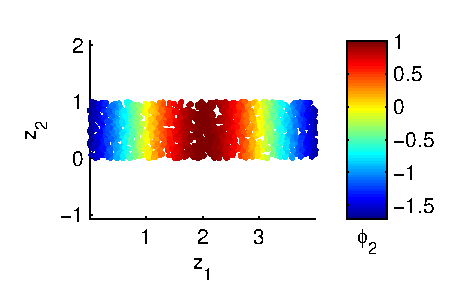
\includegraphics[width=\textwidth]{strip_discrete2}
\end{subfigure}

\begin{subfigure}{0.45\textwidth}
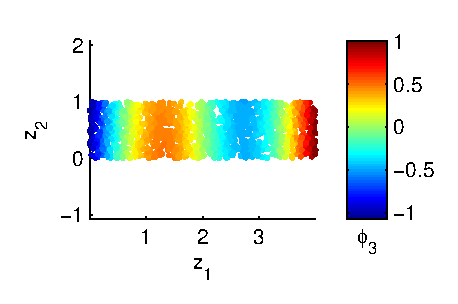
\includegraphics[width=\textwidth]{strip_discrete3}
\end{subfigure}
%
\begin{subfigure}{0.45\textwidth}
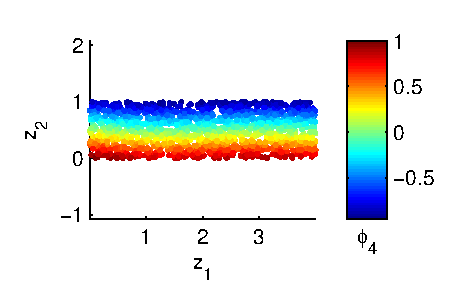
\includegraphics[width=\textwidth]{strip_discrete4}
\end{subfigure}
\caption{ Two-dimensional strip with uniform sampling colored by the first four (non-trivial) eigenvectors from diffusion maps. Note that the first and fourth eigenvectors are one-to-one with $z_1$ and $z_2$, respectively. However, the second and third eigenvectors are higher harmonics of the first eigenvector and do not capture any additional structure within the data set. }
\label{fig:strip_harmonics}
\end{figure}


Given the eigenvectors $\phi_1, \phi_2, \dots, \phi_{m-1} \in \mathbb{R}^m$, we would like to automatically deduce which ones capture new directions in the data, and which ones are merely repeated eigendirections. 
%
This problem was addressed previously in \cite{...} by performing successive iterations of diffusion maps, interspersed with advection along the first eigendirection at each iteration. 
%
However, both the advection procedure and the successive eigendecompositions are very expensive and intractable for larger data set. 
TODO: elaborate on their method and find other advantages of our proposed method (for example, theirs is ad hoc). 
%
Here, we propose an alternative approach to address the problem of repeated eigendirections. 
%
We will attempt to fit a function $f(\phi_1, \dots, \phi_{k-1})$ to $\phi_{k}$. 
%
Our approach is motivated by simple trigonometric arguments, such as $\cos2x$ can be written as a function of $\cos x$. 
%
Thus, if the resulting fit is accurate, then we assume $\phi_{k}$ is a repeated eigendirection of $\phi_1, \dots, \phi_{k-1}$. 
%
We will use a local linear function 
\begin{equation}
\phi_k \approx \alpha + \beta^T \Phi_{k-1}
\end{equation}
%
as our functional approximation, where 
%
$\Phi_{k-1} = \begin{bmatrix} \phi_1 & \dots & \phi_{k-1} \end{bmatrix}^T$,
$\alpha \in \mathbb{R}$, and $\beta \in \mathbb{R}^{k-1}$. 
%
The coefficients $\alpha$ and $\beta$ are functions of $\Phi_{k-1}$ because we use a {\em local} linear fit in the $k-1$-dimensional $\Phi_{k-1}$ space, and so the coefficients change as a function of the domain. 

At each point $\Phi_{k-1}(i)$, we approximate $\phi_k(i)$ by fitting a local linear function using the remaining $m-1$ data points. 
%
We solve the following optimization problem 
\begin{equation} \label{eq:opt_problem}
\hat{\alpha}_k (i) , \hat{\beta}_k(i)  = \argmin_{\alpha, \beta} \sum_{j \ne i} K(\Phi_{k-1}(i), \Phi_{k-1}(j)) \left( \phi_{k}(j) - (\alpha + \beta^T \Phi_{k-1}(j)) \right)^2.
\end{equation}
%
where $K$ is a kernel weighting function.
%
We will use a Gaussian kernel, 
%
\begin{equation}
K(\Phi_{k-1}(i), \Phi_{k-1}(j))  = \exp \left( - \frac{\|\Phi_{k-1}(i) - \Phi_{k-1} (j) \|^2}{\epsilon_{reg}^2} \right),
\end{equation}
%
where $\epsilon_{reg}$ is the kernel scale. 
%
We typically take $\epsilon_{reg} = M / 3$, where $M$ is the median of the pairwise distances between $\Phi_{k-1}(i)$, as we empirically found this choice to yield good results. 
%
We then define the normalized leave-one-out cross-validation error for this local linear fit as
\begin{equation} \label{eq:cv_error}
r_{k} = \sqrt{ \frac{\sum_{i=1}^n \left( \phi_{k} (i) - (\hat{\alpha}_k(i) + \hat{\beta}_k(i)^T \Phi_{k-1}(i))  \right)^2} {\sum_{i=1}^n  \left( \phi_{k} (i) \right)^2 }}
\end{equation}
%
Note that a small value of $r_k$ implies that $\phi_{k}$ can be accurately approximated from $\phi_1, \dots, \phi_{k-1}$. We will assume it means that $\phi_k$ is a harmonic of previous modes, i.e., a repeated eigendirction.
%
Conversely, a large value of $r_{k}$ indicates that $\phi_{k}$ parameterizes a new direction in the data.
%
We choose to set $r_1 = 1$.

The error in \eqref{eq:cv_error} can easily be computed \cite{wasserman2006all}.
%
We begin by computing the matrix
\begin{equation}
X_{k-1}(i) = \begin{bmatrix}
1 & \phi_1(1) - \phi_1(i) & \dots & \phi_{k-1}(1)- \phi_{k-1}(i) \\
1 & \phi_1(2) - \phi_1(i) & \dots & \phi_{k-1}(2)- \phi_{k-1}(i) \\
\vdots & \vdots & \ddots & \vdots \\
1 & \phi_1(m) - \phi_1(i) & \dots & \phi_{k-1}(m)- \phi_{k-1}(i) 
\end{bmatrix}
\end{equation}
%
and the matrix 
\begin{equation}
W_{k-1}(i) = diag \left( K(\Phi_{k-1}(i), \Phi_{k-1}(1)), \dots, K(\Phi_{k-1}(i), \Phi_{k-1}(m)) \right).
\end{equation}
%
We then calculate the smoothing matrix $L_{k-1} \in \mathbb{R}^{m \times m}$, where 
\begin{equation}
L_{k-1} =
\begin{bmatrix}
e_1^T \left( X_{k-1}^T(1) W_{k-1}(1) X_{k-1}(1) \right) ^{-1} X_{k-1}^T(1) W_{k-1}(1) \\
e_1^T \left( X_{k-1}^T(2) W_{k-1}(2) X_{k-1}(2) \right) ^{-1} X_{k-1}^T(2) W_{k-1}(2) \\
\vdots \\
e_1^T \left( X_{k-1}^T(m) W_{k-1}(m) X_{k-1}(m) \right) ^{-1} X_{k-1}^T(m) W_{k-1}(m) \\
\end{bmatrix},
\end{equation}
%
where $e_1^T = (1, 0, \dots, 0)$. 
%
We can then write
%
\begin{equation} 
r_{k} = \sqrt{ \frac{\sum_{i=1}^n \left( \frac{ \phi_{k} (i) - \sum_{j=1}^m L_{k-1}(i,j) \phi_{k}(j) }{1-L_{k-1}(i,i)} \right)^2} {\sum_{i=1}^n  \left( \phi_{k} (i) \right)^2 }} .
\end{equation}

\subsection{Calculating the relative lengths of the manifold} \label{sec:relative_lengths}

For the strip example, once the eigenvectors which parameterize unique eigendirections along the manifold have been determined, the corresponding eigenvalues can be used to calculate the relative lengths along these directions. 
%
For more general manifolds, we believe the eigenvalues can still provide a measure of the relative significance of the unique eigendirections.
%
Let $\mu_{i_1}, \mu_{i_2}, \dots$ denote the eigenvalues corresponding to eigenvectors which parameterize unique eigendirections (i.e., those eigenvectors where $r_{i_j}$ is large). 
%
For the strip example, from \eqref{eq:evals} and \eqref{eq:evals_relationship}, we propose to approximate the relative lengths $L_j$  along the manifold by
\begin{equation} \label{eq:est_lengths}
L_j \propto \frac{1}{\sqrt{-\log \mu_{i_j}}}.
\end{equation}
%
This measure is used to determine how many components are required to retain most of the information within the data set.
%
For example, if $L_j$ is smaller than a predefined threshold, then this component can be disregarded. 


\subsection{Illustrative examples} \label{sec:illustrative_examples}

We will demonstrate our proposed approach on three synthetic data sets. 
%
The first data set is the two-dimensional strip discussed previously, where the eigenvalues and eigenvectors are known analytically.
%
The second and third data sets are nonlinear manifolds which demonstrate the flexibility of our approach. 

\subsubsection{Strip}

\begin{figure}[t]
\centering
\begin{subfigure}{0.3\textwidth}
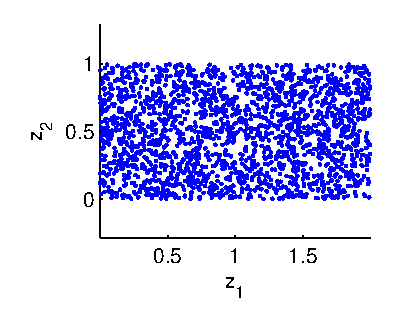
\includegraphics[height=2.5cm]{strip_data_L2}
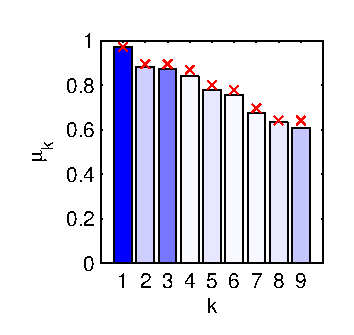
\includegraphics[height=3cm]{strip_spectrum_L2}
\caption{}
\end{subfigure}
%
\hfill
%
\begin{subfigure}{0.3\textwidth}
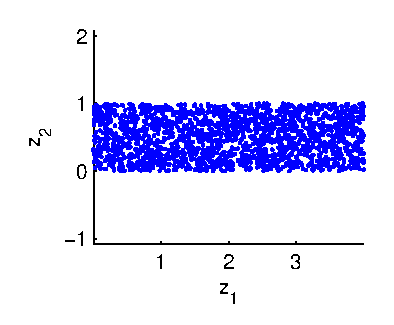
\includegraphics[height=2.5cm]{strip_data_L4}
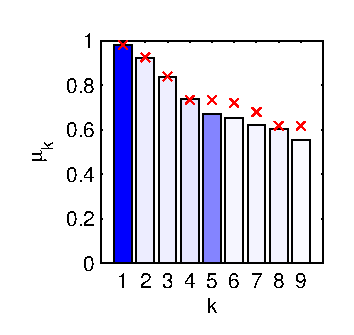
\includegraphics[height=3cm]{strip_spectrum_L4}
\caption{}
\end{subfigure}
%
\hfill
%
\begin{subfigure}{0.35\textwidth}
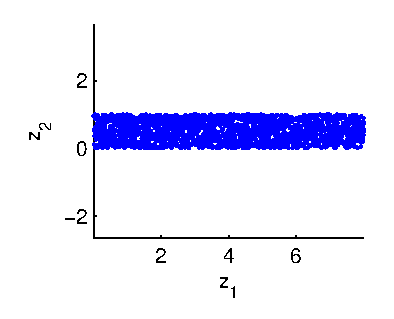
\includegraphics[height=2.5cm]{strip_data_L8}
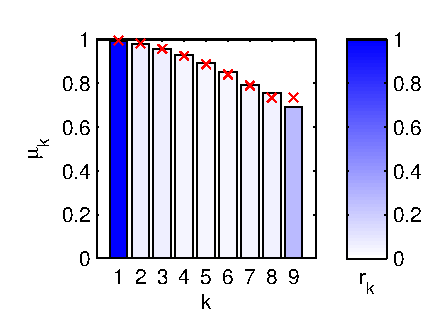
\includegraphics[height=3cm]{strip_spectrum_L8}
\caption{}
\end{subfigure}
%
\caption{Data sets (top) and eigenvalue spectra (bottom) for strips with (a) $L_1 = 2$, $L_2 = 1$, (b) $L_1 = 4$, $L_2 = 1$, (c) $L_1 = 8$, $L_2 = 1$. The empirical eigenvalues are plotted in blue, and the analytical eigenvalues are plotted in red. From the eigenvalues which are identified as important/non-harmonics, the estimated length ratio is (a) 2.2, (b) 4.1, (c) 8.7.}
\label{fig:strip_compare_analytic}
\end{figure}

Our first illustrative example consists of three different two-dimensional strip data sets. 
%
Each data set contains $m=1500$ data points uniformly sampled from the strip. 
%
Figure~\ref{fig:strip_compare_analytic} shows the data sets and corresponding eigenspectra.
%
The eigenvalues are colored by the leave-one-out cross-validation error as defined in \eqref{eq:cv_error}; a small value of $r_k$ indicate that the corresponding eigenvector is a repeated eigendirection, while a large value of $r_k$ indicates that the corresponding eigenvector describes a new direction in the data. 
%
The analytic eigenvalues of the Laplacian (see \eqref{eq:evals} and \eqref{eq:evals_relationship}) are also indicated in red. 

We observe that the eigenvalues are consistent with the known analytic eigenvalues of the Laplacian (see \eqref{eq:evals} and \eqref{eq:evals_relationship}).
%
Furthermore, the two unique eigendirections can be identified, since their corresponding regression error $r_k$ is large. 
%
As expected, we observe that the gap between the two meaningful eigenvalues increases as the strip becomes longer. 
%
Using \eqref{eq:est_lengths}, we can accurately estimate the relative lengths of the two unique eigendirections in each data set. 


\subsubsection{Swiss roll}

\begin{figure}[!th]
%
\begin{subfigure}{0.45\textwidth}
\centering
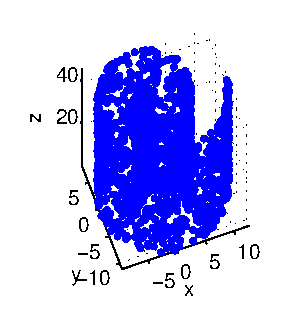
\includegraphics[height=1.25in]{swissroll1}
\caption{}
\end{subfigure}
\hfill
\begin{subfigure}{0.45\textwidth}
\centering
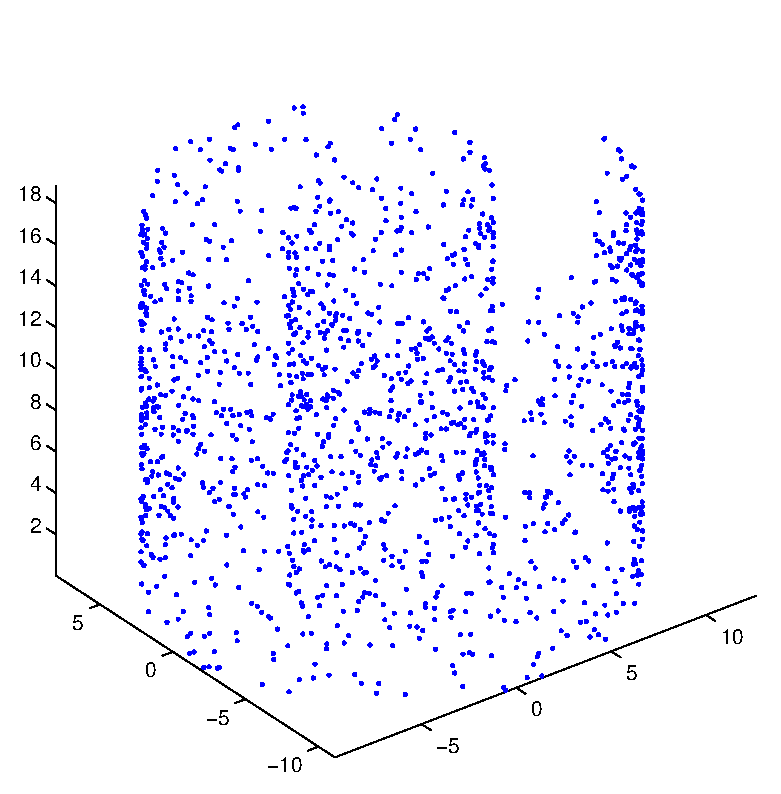
\includegraphics[height=1.25in]{swissroll2}
\caption{}
\end{subfigure}
\hfill
\begin{subfigure}{0.45\textwidth}
\centering
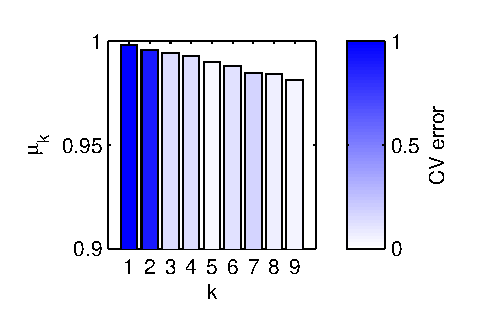
\includegraphics[height=1.25in]{swissroll1_evals}
\caption{}
\end{subfigure}
\hfill
\begin{subfigure}{0.45\textwidth}
\centering
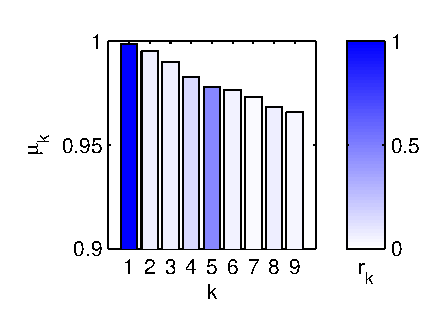
\includegraphics[height=1.25in]{swissroll2_evals}
\caption{}
\end{subfigure}
\hfill
\begin{subfigure}{0.45\textwidth}
\centering
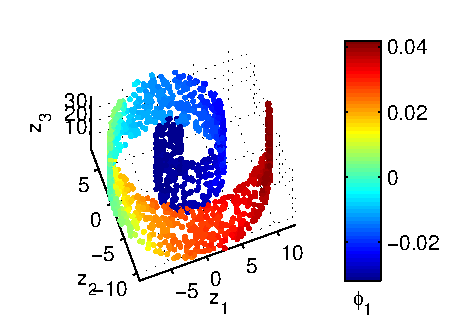
\includegraphics[height=1.25in]{swissroll1_color1} 
\caption{}
\end{subfigure}
\hfill
\begin{subfigure}{0.45\textwidth}
\centering
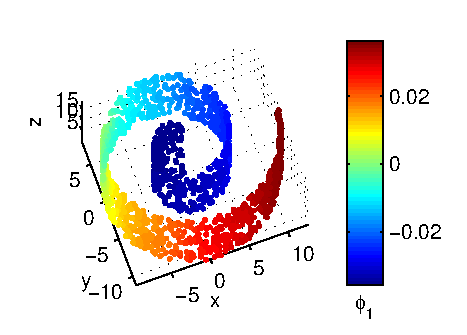
\includegraphics[height=1.25in]{swissroll2_color1}
\caption{}
\end{subfigure}
\hfill
\begin{subfigure}{0.45\textwidth}
\centering
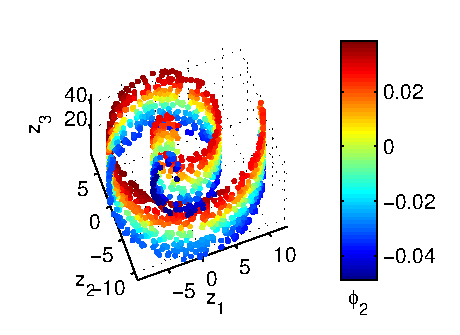
\includegraphics[height=1.25in]{swissroll1_color2}
\caption{}
\end{subfigure}
\hfill
\begin{subfigure}{0.45\textwidth}
\centering
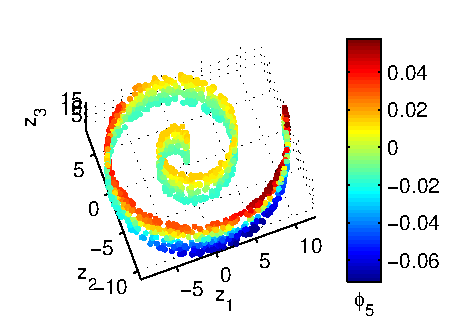
\includegraphics[height=1.25in]{swissroll2_color2}
\caption{}
\end{subfigure}
%
\caption{Swiss roll example. (a) Data set 1; $h= 40$. (b) Data set 2; $h = 20$. (c) Eigenvalue spectrum from the analysis of data set 1. (d) Eigenvalue spectrum from the analysis data set 2. (e) Data set 1, colored by the first eigenvector. (f) Data set 2, colored by the first eigenvector. (g) Data set 1, colored by the second eigenvector. (h) Data set 2, colored by the fifth eigenvector. } 
\label{fig:swiss_rolls}	
\end{figure}

Our second illustrative example consists of two different swiss roll data sets.
%
The data are sampled according to
\begin{equation}
\begin{aligned}
z_1 =& \theta \cos \theta \\
z_2 =& \theta \sin \theta \\
z_3 =& h t
\end{aligned}
\end{equation}
%
such that $z_1, z_2$ are uniformly sampled along the arclength of the spiral, and $t \sim Unif(0,1)$. 
%
Note that, in this example, $z_1, z_2, z_3$ are the original coordinates; however, the data lie on a two-dimensional manifold parameterized by the $\theta$ and $t$. 
%
The height of the first swiss roll is $h = 40$, while the height of the second is $h = 20$. 
%
Each data set consists of $m=1500$ points, shown shown in Figure~\ref{fig:swiss_rolls}(a)~and~(b).
%
%We expect to recover the eigenvector which parameterizes the height farther down in the spectrum for the second data set relative to the first, as this second data set is shorter.

Figure~\ref{fig:swiss_rolls}~(c)~and~(d) shows the eigenvalue spectra from the analysis of the two data sets.
%
Similar to Figure~\ref{fig:strip_compare_analytic}, the bars are colored by the leave-one-out cross-validation error, where a small value of $r_k$ indicates that the corresponding eigenvector is a repeated eigendirection. 
%
From these plots, one can conclude that the first two eigenvectors $\phi_1$ and $\phi_2$ parameterize the first data set, while $\phi_1$ and $\phi_5$ parameterize the second. 
%
Figure~\ref{fig:swiss_rolls}~(e--h) shows the two data sets, colored by the two eigenvectors identified by our method as parameterizing the unique eigendirections. 
%
As expected, these eigenvectors are one-to-one with the arc length along the spiral, and the height of the swiss roll. 

\subsubsection{Torus}

\begin{figure}[t]
%
\begin{subfigure}{0.3\textwidth}
\centering
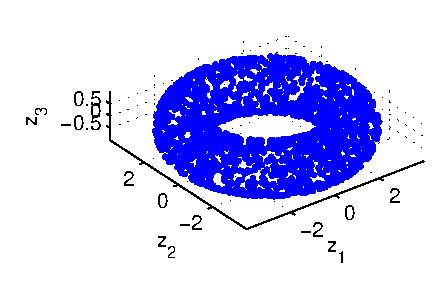
\includegraphics[height=0.75in]{torus1}
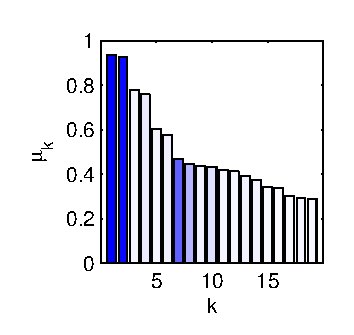
\includegraphics[height=1in]{torus1_evals}
\caption{}
\end{subfigure}
%
\hfill
%
\begin{subfigure}{0.32\textwidth}
\centering
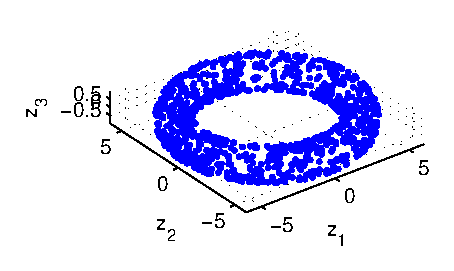
\includegraphics[height=0.75in]{torus2}
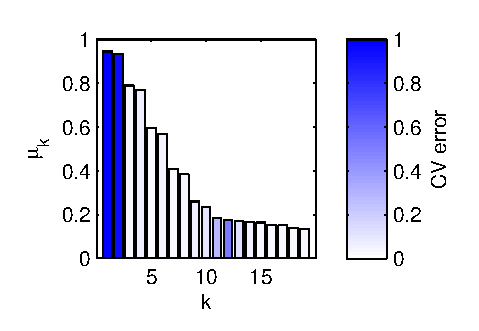
\includegraphics[height=1in]{torus2_evals}
\caption{}
\end{subfigure}
%
\hfill
%
\begin{subfigure}{0.35\textwidth}
\centering
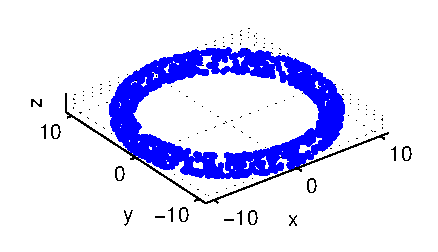
\includegraphics[height=0.75in]{torus3}
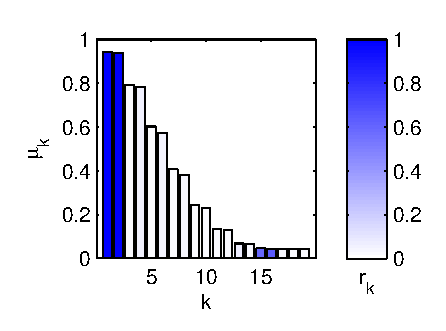
\includegraphics[height=1in]{torus3_evals}
\caption{}
\end{subfigure}
%
\hfill
%
\caption{Torii data sets (left) and corresponding eigenvalues (right). (a) $r_1 = 3$, $r_2 = 1$. (b) $r_1 = 5$, $r_2 = 1$. (c) $r_1 = 10$, $r_2 = 1$. In all three data sets, the first two eigenvalues/eigenvectors correspond to $\sin \theta_1$ and $\cos \theta_1$. The second pair of unique eigendirections (corresponding to $\sin \theta_2$ and $\cos \theta_2$) are captured by components 7 and 8, 11 and 12, and 15 and 16, respectively.}
%
\label{fig:torus}
%
\end{figure}

For the third example, we consider a torus defined by
%
\begin{equation}
\begin{aligned}
z_1 =& (r_1 + r_2 \cos \theta_2 ) \cos \theta_1 \\
z_2 =& (r_1 + r_2 \cos \theta_2 ) \sin \theta_1 \\
z_3 =& r_2 \sin \theta_2
\end{aligned}
\end{equation}
%
where $r_1 > r_2$ are the outer and inner radii, respectively, and $\theta_1, \theta_2 \sim Unif(0, 2 \pi)$. 
%
In this example, $z_1, z_2, z_3$ are the coordinates of the data; however, we expect to obtain from our analysis two eigenfunctions ($\sin \theta_1$ and $\cos \theta_1$) which parameterize the outer circle, and two eigenfunctions ($\sin \theta_2$ and $\cos \theta_2$) which parameterize the inner circle. 
%
Intuitively, increasing $r_1$ makes the eigendirections which parameterize the outer circle ($\cos \theta_1$ and $\sin \theta_1$) more dominant compared to the eigendirections with parameterize the inner circle.
%
Increasing $r_1$ can be viewed as analogous to increasing the ratio of $L_1$ to $L_2$ in the strip example. 

Figure~\ref{fig:torus} shows the eigenspectra from the analysis of three different torii, colored by the leave-one-out cross-validation error. 
%
We observe that as the torus becomes thinner ($r_1$ increases), the second pair of eigenvalues corresponding to unique eigendirections (corresponding to $\sin \theta_2$ and $\cos \theta_2$) moves farther down in the spectrum. 

\section{Chemotaxis: A Case Study}

Our main motivation for identifying the unique eigendirections is to facilitate the analysis of complex data sets where the underlying structure is not readily apparent. 
%
In data from complex dynamical systems, noisy microscopic behavior often gives rise to cohernt macroscopic dynamics. 
%
%Although on the microscale the system consists of many stochastic and noisy particles, it exhibits coherent dynamics on the macroscale which are governed by only a few parameters.
%
In general, this mapping from microscale to macroscale is not always obvious.
%
We will show how we can use our proposed methodology to extract a parameterization of data collected at the microscale which is consistent with the macroscopic behavior, without any {\em a priori} knowledge of the appropriate microscopic or macroscopic model.
%
Furthermore, determining the {\em true} dimensionality of such a parameterization by identifying the unique eigendirections in the analysis uncovers the requisite dimensionality of a reduced model which captures the relevant macroscopic behavior. 
%
Knowing appropriate macroscopic variables and the true dimensionality can help inform modeling efforts and aid in the writing of accurate macroscale models.



%For example, fluid flow, which can be described via the position and velocity of every fluid particle, is modeled at the macroscale using the Navier-Stokes equations.
%

%In this letter, we will demonstrate how this goal can be achieved through a data-driven method based on geometric analysis and manifold learning. 
%
%Specifically, we aim to emphasize two particular aspects of manifold learning from a dynamical systems' point of view: (a) choosing the appropriate observers, especially in presence of stochastic dynamics, and (b) selecting an appropriate metric for comparison \cite{mallat2012group}. 
%
%We will show that both are essential for data-driven algorithms to successfully uncover the underlying system dynamics. 

Our model problem describes the process of cellular chemotaxis \cite{othmer2000diffusion}, where biological cells exhibit coherent macroscopic dynamics regulated by extracellular sensed signals in order to accomplish tasks such as finding food or navigating away from toxins.
%
Several microscopic models have been proposed to describe chemotaxis dynamics \cite{othmer1988models, codling2008random}.
%
We will analyze one such model described by a one-dimensional velocity jump process \cite{othmer2000diffusion}.
%
%In this model, each cell is initialized with a position and a velocity on a line, and the dynamics of each cell are governed by a stochastic process.
%
%At random times, a cell will ``turn around'' and switch the direction of its velocity (this turning is controlled by extracellular signals). 
%
%We will analyze the dynamics of collections of such cells/particles. 
%
%In this example, the macroscopic dynamics of the group of cells vary depending on the value of a single system parameter.
%
%We will demonstrate how we can use diffusion maps \cite{coifman2005geometric}, a manifold learning technique, to {\em automatically} detect changes in the system's macroscopic dynamics from microscale data.
%
%This case study exhibits several key points which allow us to demonstrate the strength of our diffusion maps approach.
%
%First, this system has random microscopic behavior with smooth macroscopic dynamics governed by a single parameter which determines the regime/mode of the system. 
%
%Second, it consists of an ensemble of individual stochastic particles which must be described using the appropriate observers.
%
%Third, it has an analytic macroscopic description, which serves as a ground truth and will allow us to verify our results which are obtained in an unsupervised manner.
This specific example has an analytic macroscopic description in which the macroscopic dynamics of the group of cells depend on the value of a single system parameter.
%
This model serves as a ground truth and will allow us to verify our results which are obtained in an unsupervised manner.
%
Thus far, we only considered synthetic data sets for which the Euclidean distance between data points served as an informative metric. 
%
Here, we will show that our approach, when utilizing the appropriate statistical observers and affinity metric between pairs of observations, uncovers a parameterization of the microscopic data which is consistent with the macroscopic model.
%
Furthermore, we will show that changes in dynamical behavior resulting from changes in the system parameters can be automatically detected. 

%The remainder of this letter is organized as follows. 
%
%We begin by describing the chemotaxis problem, the illustrative example used to demonstrate the methodologies.
%%
%We present the stochastic microscopic model, and use diffusion maps, a nonlinear dimensionality reduction technique, to analyze microscopic simulation results.
%%
%We show that the governing macroscopic variables can be recovered, provided that the appropriate observers and distance metric are used.
%%
%We then describe how, for this example, the microscopic model gives rise to a compact macroscopic description governed by a single parameter, and show that the diffusion maps results are consistent with this macroscopic description. 
%%
%Finally, we demonstrate that diffusion maps can also identify the relative importance of system variables in different parameter regimes, and detect changes in macroscopic dynamical behavior.

%\section{Problem formulation}

%\subsection{Chemotaxis ``story''} 


\subsection{Problem description}

The microscopic model consists of a collection of $N$ cells (for our simulations, we take $N=1000$) whose states are defined by their positions and velocities on a line, and the dynamics of each cell are governed by a stochastic process.
%
Let $x_i(t)$ and $v_i(t)$ denote the position and velocity, respectively, of cell $i$ at time $t$.
%
The velocity of each cell is $\pm s$, where $s$ is a (fixed) speed. 
%
We initialize the cells such that
\begin{equation}\label{eqn:system}
\begin{aligned}
x_i(0) & = 0 \\
\mathbb{P} \{ v_i(0) = +s \} & = p
\end{aligned}
\end{equation}
where $0 < p < 1$ is the probability of a cell initially moving to the right.
%
At random times, a cell will ``turn around'' and switch the direction of its velocity (this turning is controlled by extracellular signals). 
%
The velocity of each cell randomly switches between $\pm s$ following an (independent) Poisson process with rate $\lambda$.
%
For our specific simulations, we set $s^2/\lambda=1$, which is consistent with the analysis presented in \cite{...}. 
%
We note that we have chosen a very specific one-parameter family of initial conditions which lead to simple dynamics and allow us to illustrate of our main points;
however, our analysis is not restricted to such specific cases and more complex initial conditions could be used. 

\subsection{Observers and metrics}

In general, manifold learning techniques have two essential components.
%
One is the appropriate {\em observers} of the system. 
%
These observers should be informative as to the state of the system, as well as insensitive to noise in the system. 
%
Two is a {\em distance metric} between the observations that captures a notion of locality: observations which we perceive to be similar should have a small distance. 
%
%For this particular example, we will use histograms of the particle positions as the observations, and the EMD as the distance metric.


%Appropriate observers can be constructed in several different ways. 
%%
%For simple data, such as the illustrative examples in Section~\ref{sec:illustrative_examples}, the observers are simply the data points themselves. 
%%
%However, for more complex data, the raw data may contain other sources of variability which are not meaningful to the system dynamics. 
%%
%For some examples, physical intuition and {\em a priori} knowledge can aid in constructing appropriate observers. 
%%
%For example, when looking at a protein, the observers may be the locations of the $\alpha$-carbons, as these backbone atoms are known to capture most of the relevant dynamics. 
%%
%Observers can also remove unimportant sources of variation; 
%for example, the bispectrum \cite{zhao2014rotationally} and the scattering transform \cite{mallat2012group} are both invariant to rotations. 
%%
%Observers should also be robust to noise, which motivates the scattering transform \cite{mallat2012group} and histograms \cite{talmon2013empirical}.
%
%After constructing appropriate observers, one must choose the appropriate metric for the diffusion maps calculation. 
%%
%The simplest option (used for the illustrative examples in Section~\ref{sec:illustrative_examples}) is to use the Euclidean distance, but this can often prove uninformative. 
%%
%For molecular simulation data, it is often appropriate to use the Euclidean distance {\em after} aligning configurations with respect to rotations, as global rotations of the entire molecule are not meaningful \cite{ferguson2010systematic}.
%%
%For dynamical systems which are obscured by large variance noise, the Mahalanobis distance often yields a more informative parameterization of the data \cite{talmon2013empirical}.
%%
%Another option is the Earth Mover's Distance, a multiscale distance metric which is stable and robust to noise \cite{rubner2000earth}.

For the chemotaxis example, we use histograms of the particle positions as observers \cite{talmon2013empirical}. 
%
Histograms are invariant to the indexing of the particles, while retaining the spatial locations of the particles.
%
The histograms are also robust to noise \cite{talmon2013empirical}. 
%
Instead of the standard Euclidean distance, we use the earth mover's distance (EMD) \cite{rubner2000earth} as the metric between pairs of histograms. 
%
Conceptually, the EMD measures how much ``work'' it takes to transform one probability density into another.
%
It therefore not only considers where the densities are inconsistent, but also how far apart the inconsistencies are.
%
Although the brute-force computation of the EMD is computationally expensive, there has been a plethora of work in developing efficient algorithms for its approximation \cite{Pele-eccv2008, Pele-iccv2009}.
%
For the special case of one-dimensional data, the EMD is equivalent to the $L_1$-norm between the cumulative distribution functions of the data \cite{rubner2000perceptual}, which can be approximated from histograms as
\begin{equation}
\| z(i) - z(j) \|_{EMD} \approx \sum_{l=1}^{n} \left| \sum_{k=1}^l z_k(i) - \sum_{k=1}^l z_k(j) \right|
\end{equation}
where the histograms $z(i), z(j)$ are defined on equally-spaced bins in $\mathbb{R}$, and $z_k$ denotes the $k^{th}$ bin. 
%
We note that although histograms are not essential for using EMD, histograms make the computation feasible. 
%
For our specific simulations, we will take $n=32$. 

%\subsubsection{Constructing appropriate observers}
%
%\begin{itemize}
%\item Physical examples (e.g., $\alpha$-carbons for molecules)
%\item Amit's bispectrum
%\item Scattering transform
%\item Cite PNAS, stating that the histograms are good since they linearize any noise. 
%For the chemotaxis example, we use histograms of the particle positions as observers \cite{talmon2013empirical}. 
%%
%Histograms are invariant to the indexing of the particles, while retaining the spatial locations of the particles.
%\end{itemize}
%
%\subsubsection{Defining a meaningful metric}
%
%
%\begin{itemize}
%\item Euclidean (not good, especially for histograms)
%\item Mahalanobis (good, cite PNAS, since it noise robust)
%\item Here we use EMD since it is multiscale.
%%
%Instead of the standard Euclidean distance, we use the earth mover's distance (EMD) \cite{rubner2000earth} as the metric between pairs of histograms. 
%%
%Conceptually, the EMD measures how much ``work'' it takes to transform one probability density into another.
%%
%It therefore not only considers where the densities are inconsistent, but also how far apart the inconsistencies are.
%%
%Although the brute-force computation of the EMD is computationally expensive, there has been a plethora of work in developing efficient algorithms for its computation \cite{Pele-eccv2008, Pele-iccv2009}.
%%
%For the special case of one-dimensional data, the EMD is equivalent to the $L_1$-norm between the cumulative distribution functions \cite{rubner2000perceptual}, which can be estimated from histograms as
%\begin{equation}
%\| z(i) - z(j) \|_{EMD} \approx \sum_{l=1}^{n} \left| \sum_{k=1}^l z_k(i) - \sum_{k=1}^l z_k(j) \right|
%\end{equation}
%where the histograms $z(i), z(j)$ are defined on equally-spaced bins in $\mathbb{R}$, and $z_k$ denotes the $k^{th}$ bin. 
%%
%\item Emphasize stability and regularity issues.
%\end{itemize}






\subsection{Results}

\subsubsection{Identifying the unique eigendirections}

\begin{figure}[t!]
\def \figwidth {3.5cm}

\centering
\begin{subfigure}{\figwidth}
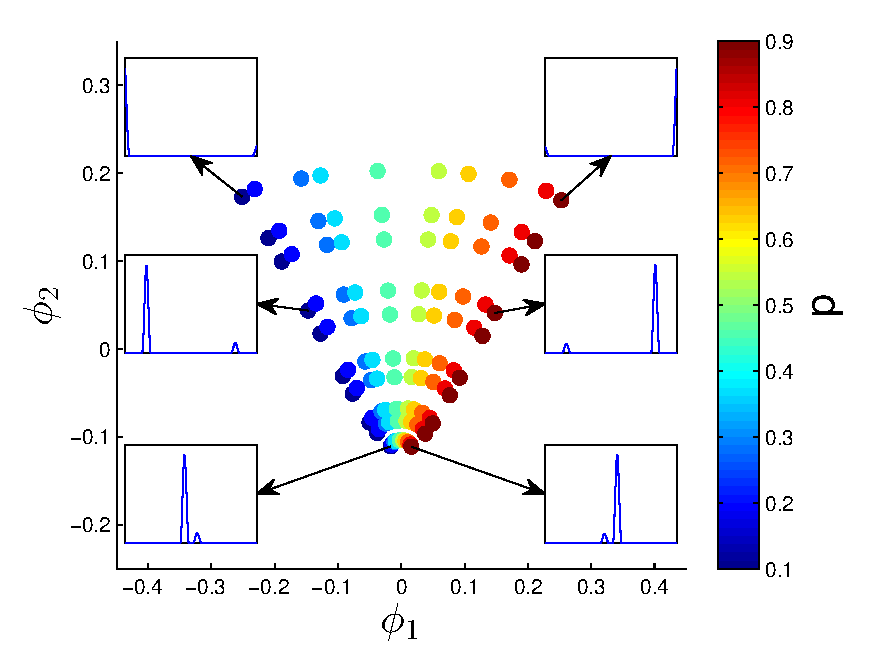
\includegraphics[width=\textwidth]{EMD_withhist_p_1}
\caption{}
\label{subfig:small_lambda_p}
\end{subfigure}
\begin{subfigure}{\figwidth}
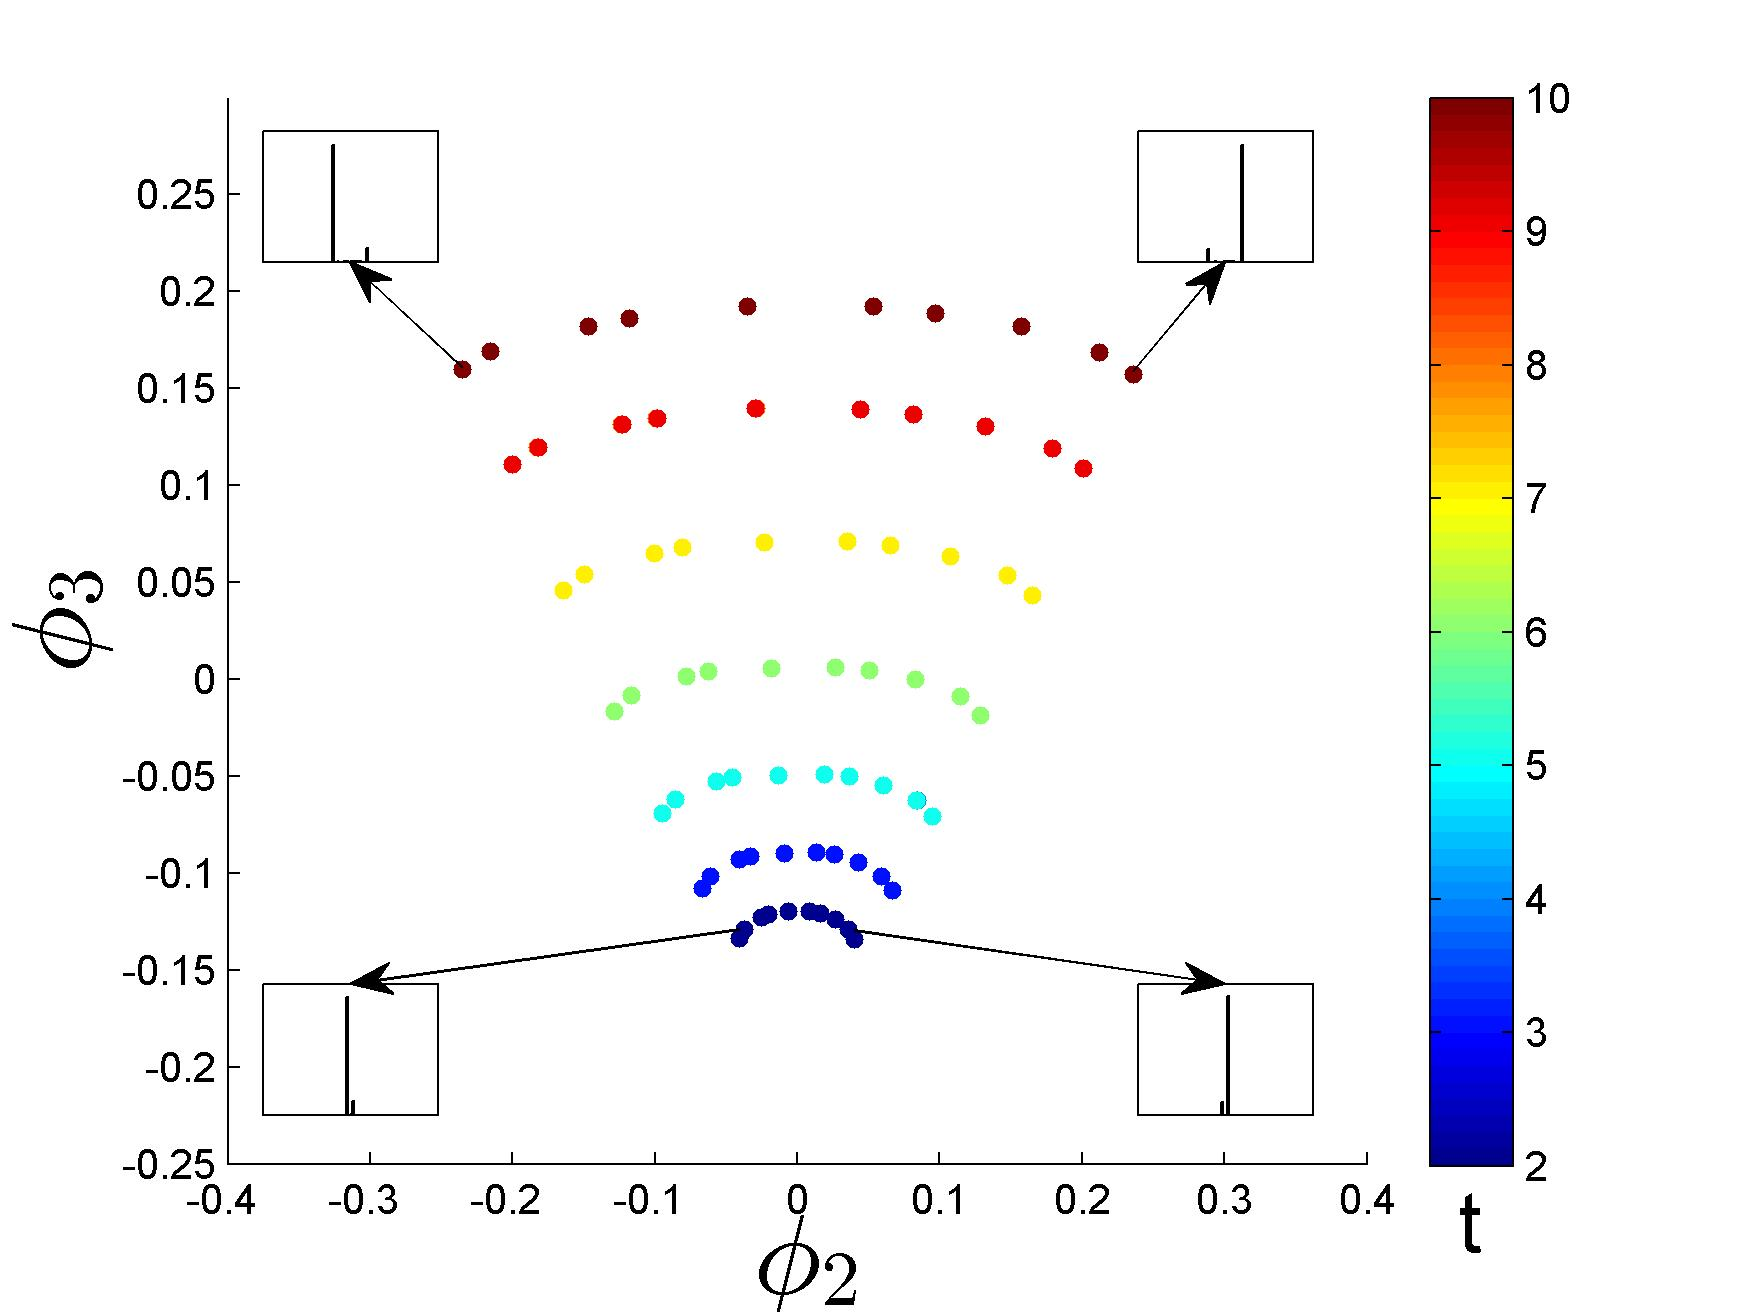
\includegraphics[width=\textwidth]{EMD_withhist_t_1}
\caption{}
\label{subfig:small_lambda_t}
\end{subfigure}
\begin{subfigure}{\figwidth}
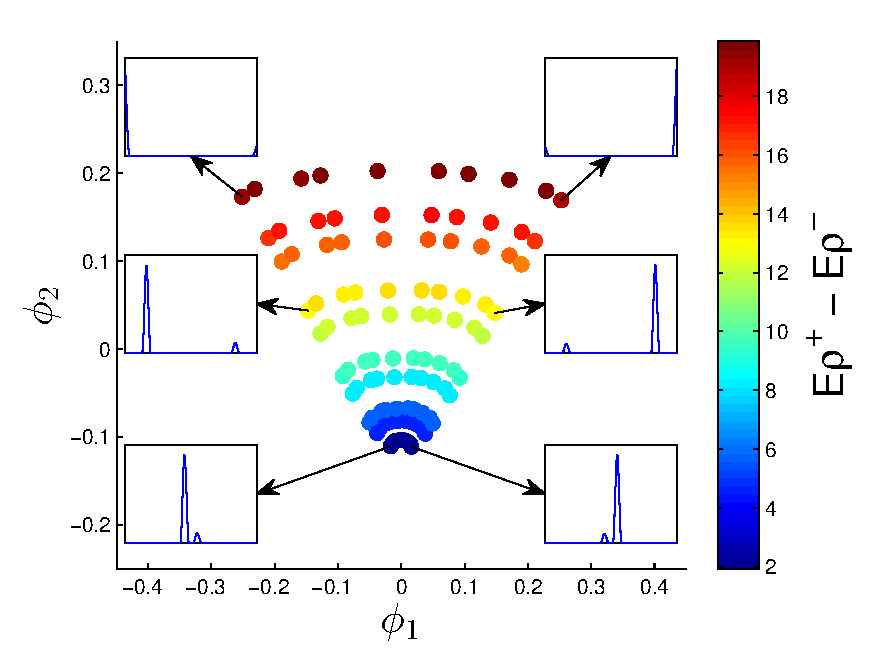
\includegraphics[width=\textwidth]{EMD_withhist_rho_1}
\caption{}
\label{subfig:small_lambda_rho}
\end{subfigure}

\begin{subfigure}{\figwidth}
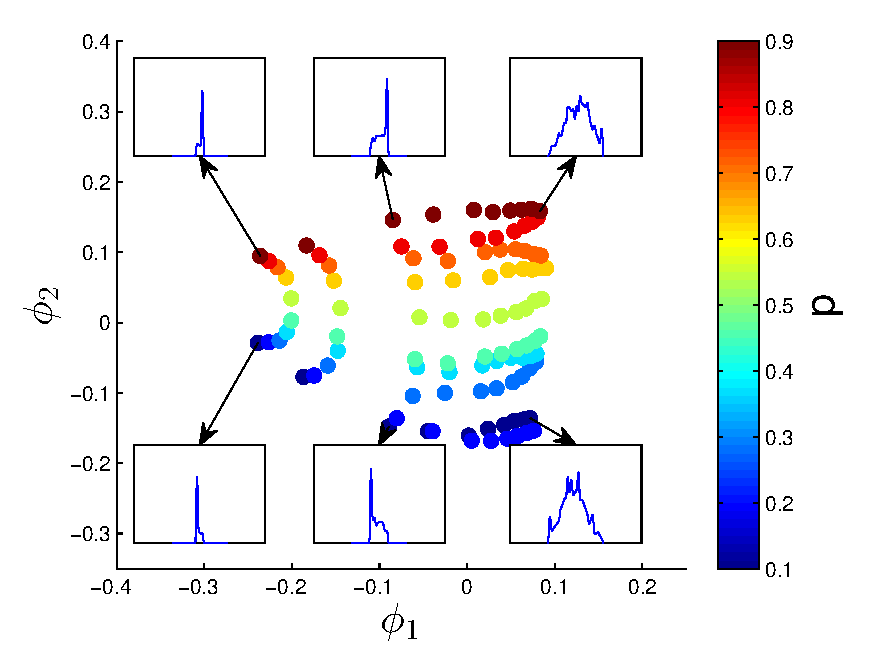
\includegraphics[width=\textwidth]{EMD_withhist_p_400}
\caption{}
\label{subfig:large_lambda_p}
\end{subfigure}
\begin{subfigure}{\figwidth}
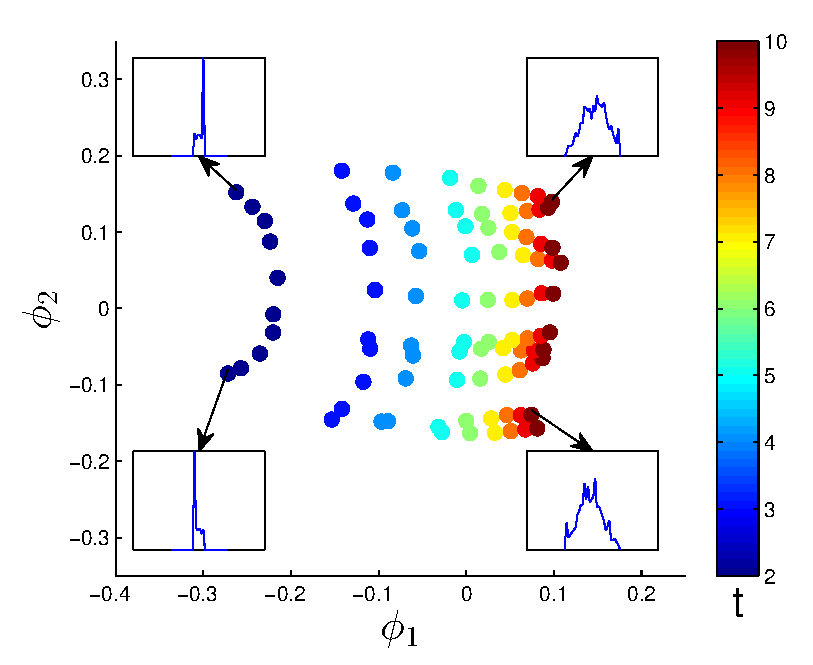
\includegraphics[width=\textwidth]{EMD_withhist_t_400}
\caption{}
\label{subfig:large_lambda_t}
\end{subfigure}
\begin{subfigure}{\figwidth}
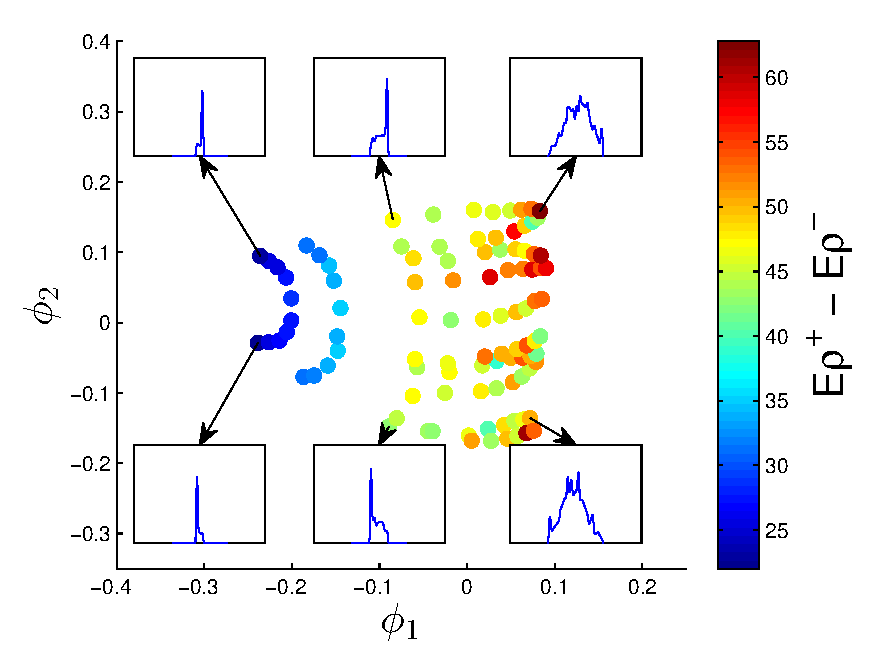
\includegraphics[width=\textwidth]{EMD_withhist_rho_400}
\caption{}
\label{subfig:large_lambda_rho}
\end{subfigure}
\caption{Diffusion maps embeddings computed from simulation data of the velocity jump process with (a--c) $\lambda=1$, $s=1$, and (d--f) $\lambda=400$, $s=20$.  Each data set consists of $10$ simulations, with initial conditions uniformly chosen such that $0.1 \le p  \le 0.9$. We allow each simulation to evolve for $10$ time units, with $dt=1$, and use data with $t > 0$ for analysis. The distances used in the diffusion maps kernel are the earth mover's distances between the histograms of particle positions. The data are colored by (a, d) $p$, the initial probability of a particle moving to the right, (b, e) $t$, time. Representative histograms are shown for selected data points, and (c, f) $E \rho^+ - E \rho^-$, the difference between the average position of the left- and right-moving particles.}
\label{fig:dmaps_embed_emd}
\end{figure}

\begin{figure}
%
\def\figheight{1.4in}
%
\begin{subfigure}[t]{0.31\textwidth}
\centering
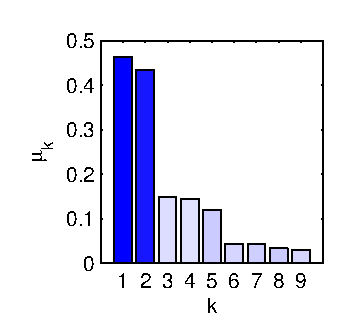
\includegraphics[height=\figheight]{chemotaxis1_evals}
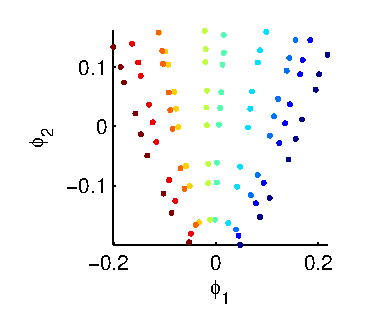
\includegraphics[height=\figheight]{chemotaxis1_embed_good}
\vspace{1.2in}
%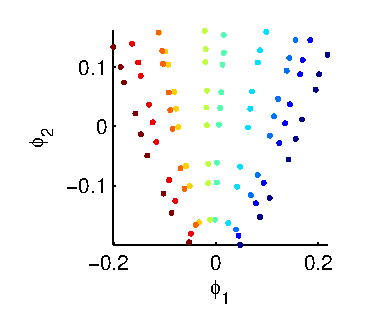
\includegraphics[height=1.5in]{chemotaxis1_embed_bad}
\caption{}
\end{subfigure}
%
\begin{subfigure}[t]{0.31\textwidth}
\centering
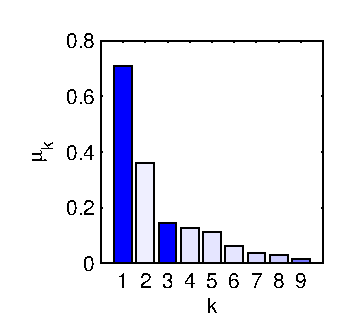
\includegraphics[height=\figheight]{chemotaxis2_evals}
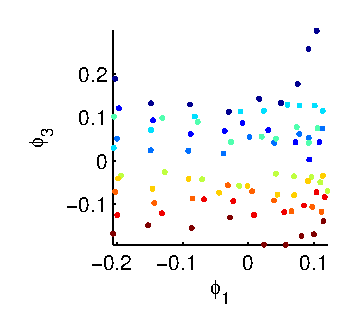
\includegraphics[height=\figheight]{chemotaxis2_embed_good}
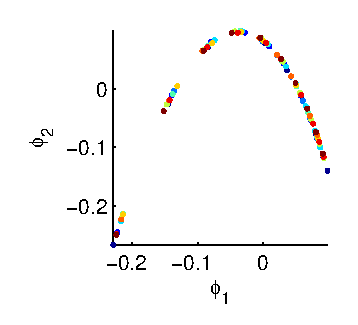
\includegraphics[height=\figheight]{chemotaxis2_embed_bad}
\caption{}
\end{subfigure}
%
\begin{subfigure}[t]{0.35\textwidth}
\centering
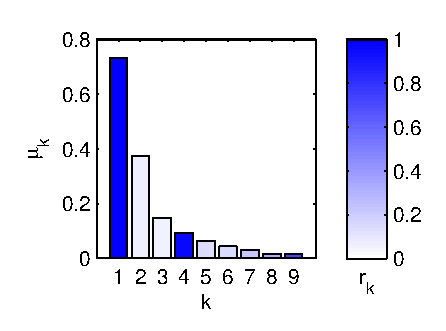
\includegraphics[height=\figheight]{chemotaxis3_evals}
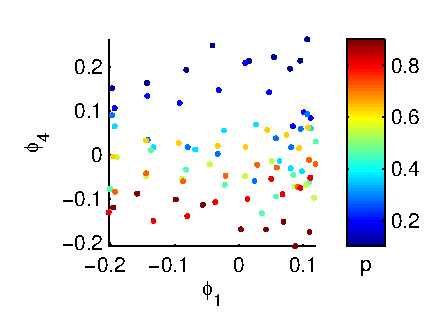
\includegraphics[height=\figheight]{chemotaxis3_embed_good}
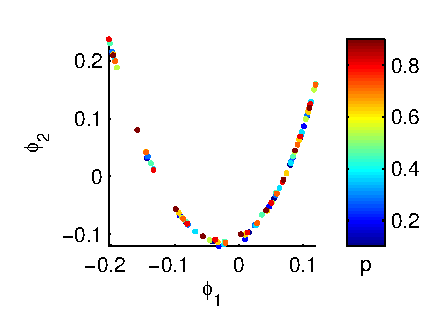
\includegraphics[height=\figheight]{chemotaxis3_embed_bad}
\caption{}
\end{subfigure}
%
\caption{Diffusion maps embedding for three different chemotaxis simulation data sets. (a) $\lambda = 100$, $s = 10$. (b) $\lambda = 1600$, $s = 40$. (c) $\lambda = 6400$, $s = 80$. Each data set consists of $10$ simulations, with initial conditions uniformly chosen such that $0.1 \le p  \le 0.9$. We allow each simulation to evolve for $10$ time units, with $dt=1$, and use data with $t > 0$ for analysis. The distances used in the diffusion maps kernel are the earth mover's distances between the histograms of particle positions. For each data set, the eigenvalue spectrum, colored by the cross-validation error, is shown. From the spectra, we can see that the first two components are informative for (a), components 1 and 3 are informative for (b), and components 1 and 4 are informative for (c). The corresponding embeddings are shown below. For comparison, the embeddings using the first two components are also shown in (b) and (c).}
%
\label{fig:chemotaxis_simulations_harmonics}
\end{figure}


Figure~\ref{fig:dmaps_embed_emd} shows the results of analyzing two sets of chemotaxis simulations. 
%
One set of simulations (Figures~\ref{subfig:small_lambda_p}--\ref{subfig:small_lambda_rho}) is for a small value of $\lambda$, and the other set (Figures~\ref{subfig:large_lambda_p}--\ref{subfig:large_lambda_rho}) is for a large value of $\lambda$. 
%
For both sets of simulations, the macroscopic variables $p$, which controls the initial distribution of the cells, and $t$, the time, are well-correlated with the eigenvectors $\phi_1$ and $\phi_2$. 
%
%In both cases, $\phi_1$ is significantly more important than $\phi_2$, as indicated by the separation between the first two eigenvalues (for the small $\lambda$ case, $\mu_1 = 0.4828$, and $\mu_2 = 0.4287$, and for the large $\lambda$ case, $\mu_1 = 0.6288$, and $\mu_2 = 0.3236$).
%
The dominant coordinate $\phi_1$ is correlated with $p$ for the small $\lambda$ case (Figure~\ref{subfig:small_lambda_p}), and correlated with $t$ for the large $\lambda$ case (Figure~\ref{subfig:large_lambda_t}), indicating that the relative importance of $p$ and $t$ changes in the two simulations.
%
TODO: should we mention fluxes here??

As illustrated in the synthetic data sets we discussed previously, the two leading eigenvectors are not guaranteed to correspond to unique eigendirections. 
%
Figure~\ref{fig:chemotaxis_simulations_harmonics} shows the results of analyzing three different simulations which span a larger range of $\lambda$ values compared to Figure~\ref{fig:dmaps_embed_emd}. 
%
We see from the eigenspectra and the cross-validation errors $r_k$ that the second unique eigendirection moves down in the spectrum as $\lambda$ increases. 
%
Plotting the data using the two eigenvectors identified as corresponding to unique eigendirections yields two-dimensional embeddings which capture the macroscopic variables $p$ and $t$ (we only show the correspondence of the two identified unique eigendirections with $p$ in the middle row of Figure~\ref{fig:chemotaxis_simulations_harmonics} and report that the correspondence between these eigendirections and $t$ is also consistent). 
%
In contrast, plotting the data using the two leading eigenvectors $\phi_1$ and $\phi_2$ produces uninformative embeddings for large values of $\lambda$, as $\phi_2$ is a repeated eigendirection which does not parameterize any new directions in the data.
%
From the top row of Figure~\ref{fig:chemotaxis_simulations_harmonics}, we can see that the eigenvalue spectrum does not exhibit any large spectral gaps.
%
However, there is a significant gap between the eigenvalues which correspond to new directions in the data (colored in blue), and the corresponding eigenvectors provide us with an informative two-dimensional parameterization of the data. %which is consistent with the expected macroscopic dynamics. 
%
It now becomes clear that looking at the eigenvectors {\em modulo} repeated eigendirections is essential for extracting an informative parameterization of the data, as well as characterizing the dimensionality of the data. 



%\subsubsection{Detecting changes in dynamical behavior}
%
%
%%\begin{figure}[t] 
%%\centering
%%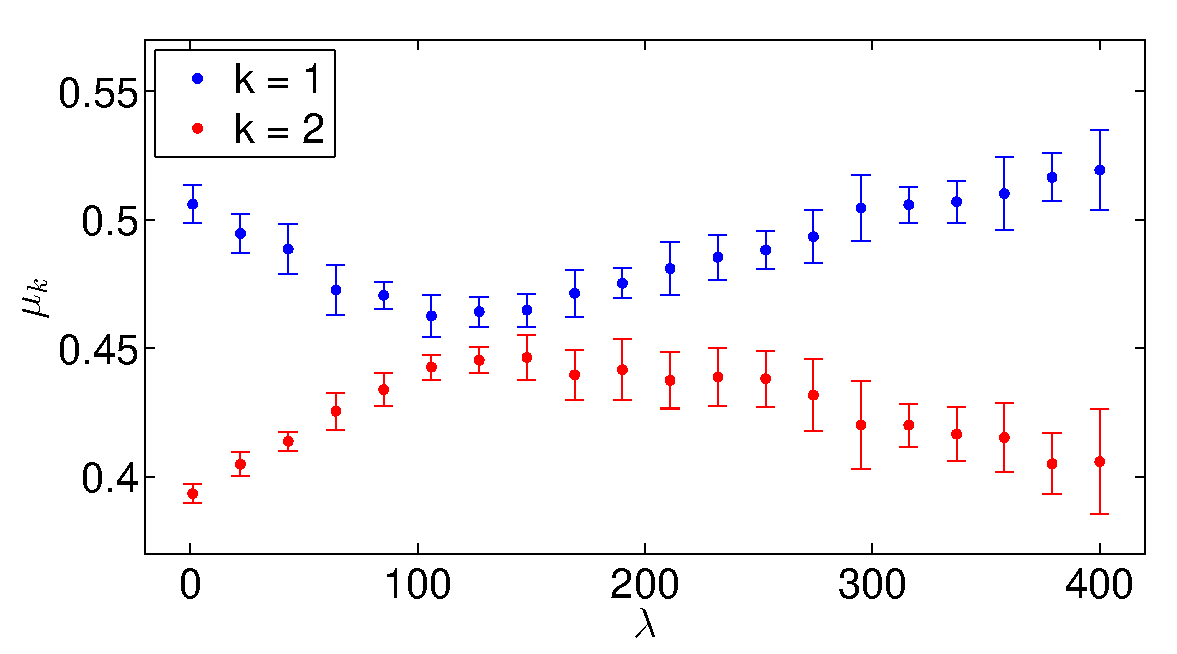
\includegraphics[width=0.5\textwidth]{detect_change_eigenvalues}
%%\caption{The first two eigenvalues from our analysis as a function of $\lambda$. Each point is averaged over $10$ experiments (as in Figure~\ref{fig:dmaps_embed_emd}, one experiment consists of data collected at varying $p$ and $t$, for a fixed value of $\lambda$), with error bars denoting one standard deviation. 
%%The convergence of the eigenvalues at $\lambda \approx 125$ indicates switching of the dynamical ``mode''.}
%%\label{fig:detect_change}
%%\end{figure}
%
%%We have seen that the eigenvalues $\mu_i$, which quantify the importance of each embedding coordinate, reveal the relative importance of the variables which govern the macroscopic dynamics.
%%
%We can use the eigenvalues from our analysis to detect changes in dynamical behavior.
%%
%From Figure~\ref{fig:dmaps_embed_emd}, we can see that the dominant eigendirection is correlated with $p$ when $\lambda$ is small, and correlated with $t$ when $\lambda$ is large. 
%%
%%We expect an intermediate $\lambda$ value where $p$ and $t$ are equally important. 
%%%
%%From the analytic macroscopic description, we expect a gap between the two eigenvalues at the two asymptotic regimes ($\lambda \rightarrow 0$, where the dynamics are described by two uncoupled wave equations \eqref{...}, and $\lambda \rightarrow \infty$, where the dynamics are described by a single heat equation \eqref{...}), as one of the two macroscopic variables is significantly more important to the dynamical behavior.
%%%
%%For intermediate $\lambda$ values, we expect the gap between $|\mu_1|$ and $|\mu_2|$ to narrow, with the $\lambda$ value where $|\mu_1| \approx |\mu_2|$ corresponding to the transition between ``wave-like'' and ``heat-like'' behavior. 
%%
%We performed a new set of simulations over a range of $\lambda$ values;  
%Figure~\ref{fig:detect_change} shows the first two eigenvalues, $\mu_1$ and $\mu_2$, from our analysis as a function of $\lambda$.
%%
%For small $\lambda$ (corresponding to Figures~\ref{subfig:small_lambda_p}~and~\ref{subfig:small_lambda_t}), the two eigenvalues are well-separated, as the first mode (which parameterizes $p$) is significantly more important than the second mode (which parameterizes $t$).
%%
%At intermediate $\lambda$ values, the eigenvalues come together as the system dynamics change and both $p$ and $t$ are of similar importance.
%%
%The eigenvalues then separate again at large $\lambda$ (corresponding to Figures~\ref{subfig:large_lambda_p}~and~\ref{subfig:large_lambda_t}), where the $t$ effects dominate the dynamics.
%%
%We can therefore detect changes in dynamical behavior using data-driven techniques, without any knowledge of the governing macroscopic model. 
%%
%In the next section, we will show that the detected changes in dynamical behavior is consistent with the analytic macroscale model.
%
%%\begin{figure}[t]
%%\def\figwidth{4.2cm}
%%\begin{subfigure}{\figwidth}
%%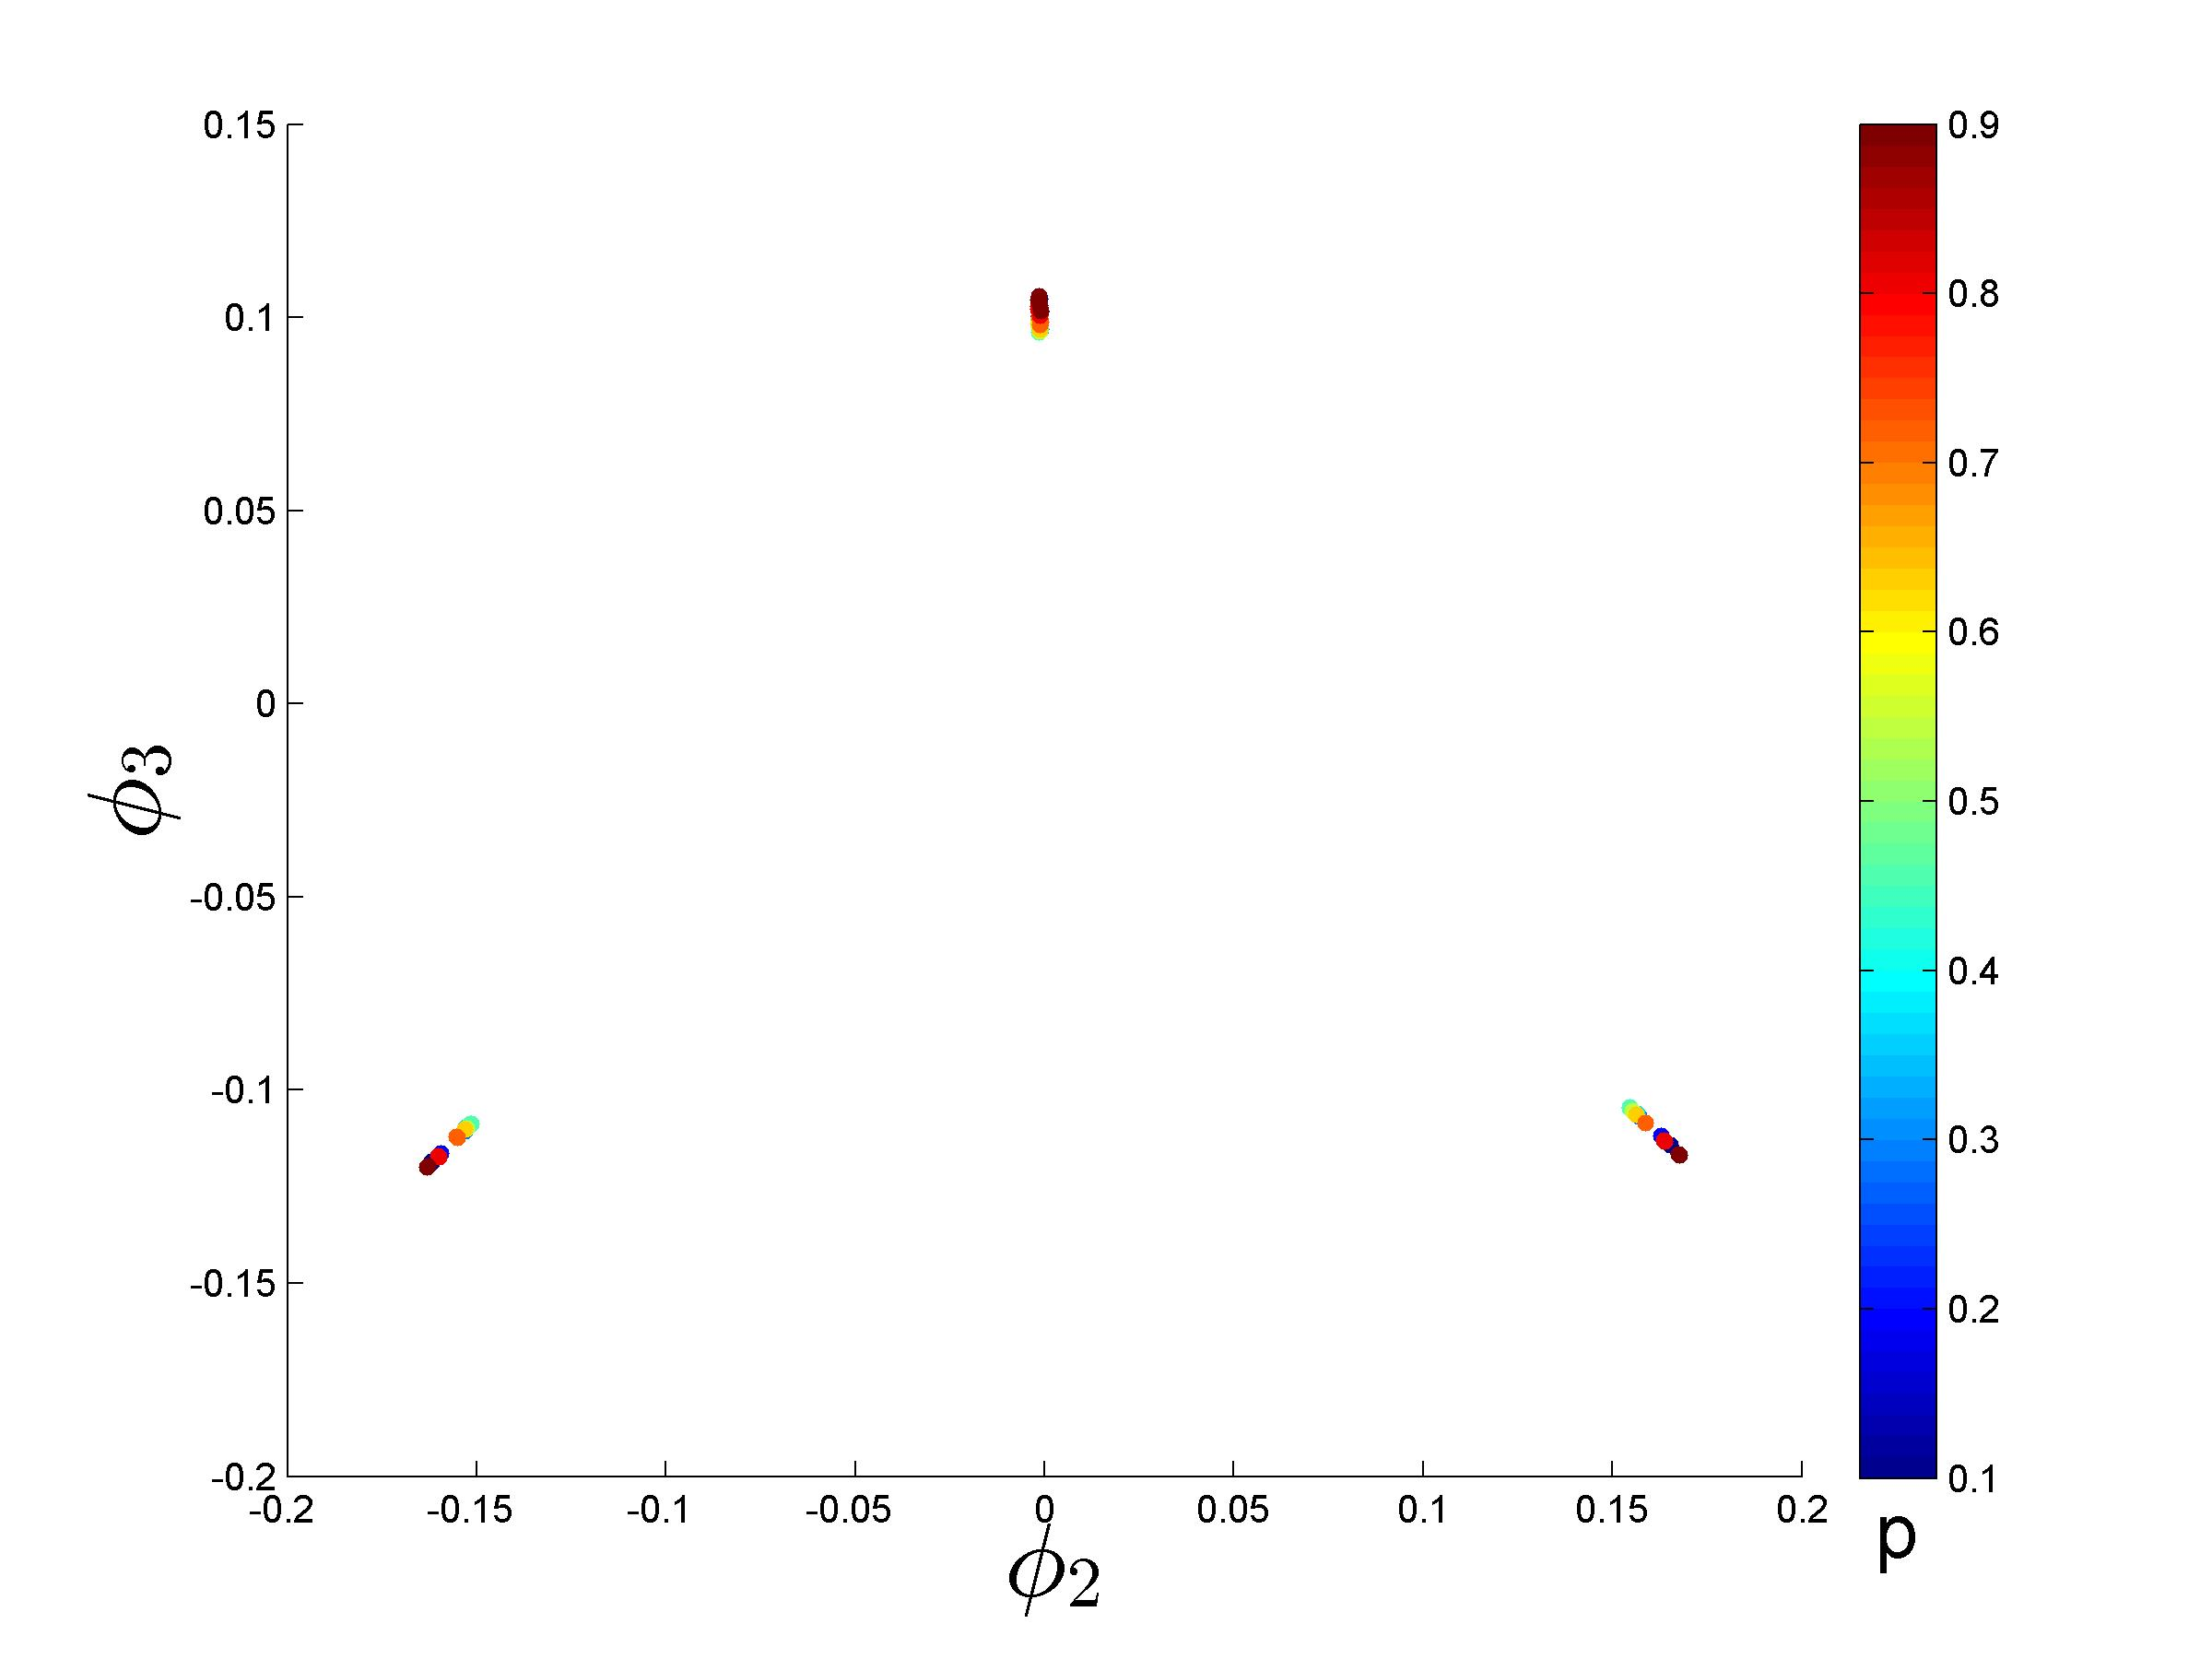
\includegraphics[width=\textwidth]{rawhist_p_1}
%%\caption{}
%%\end{subfigure}
%%\begin{subfigure}{\figwidth}
%%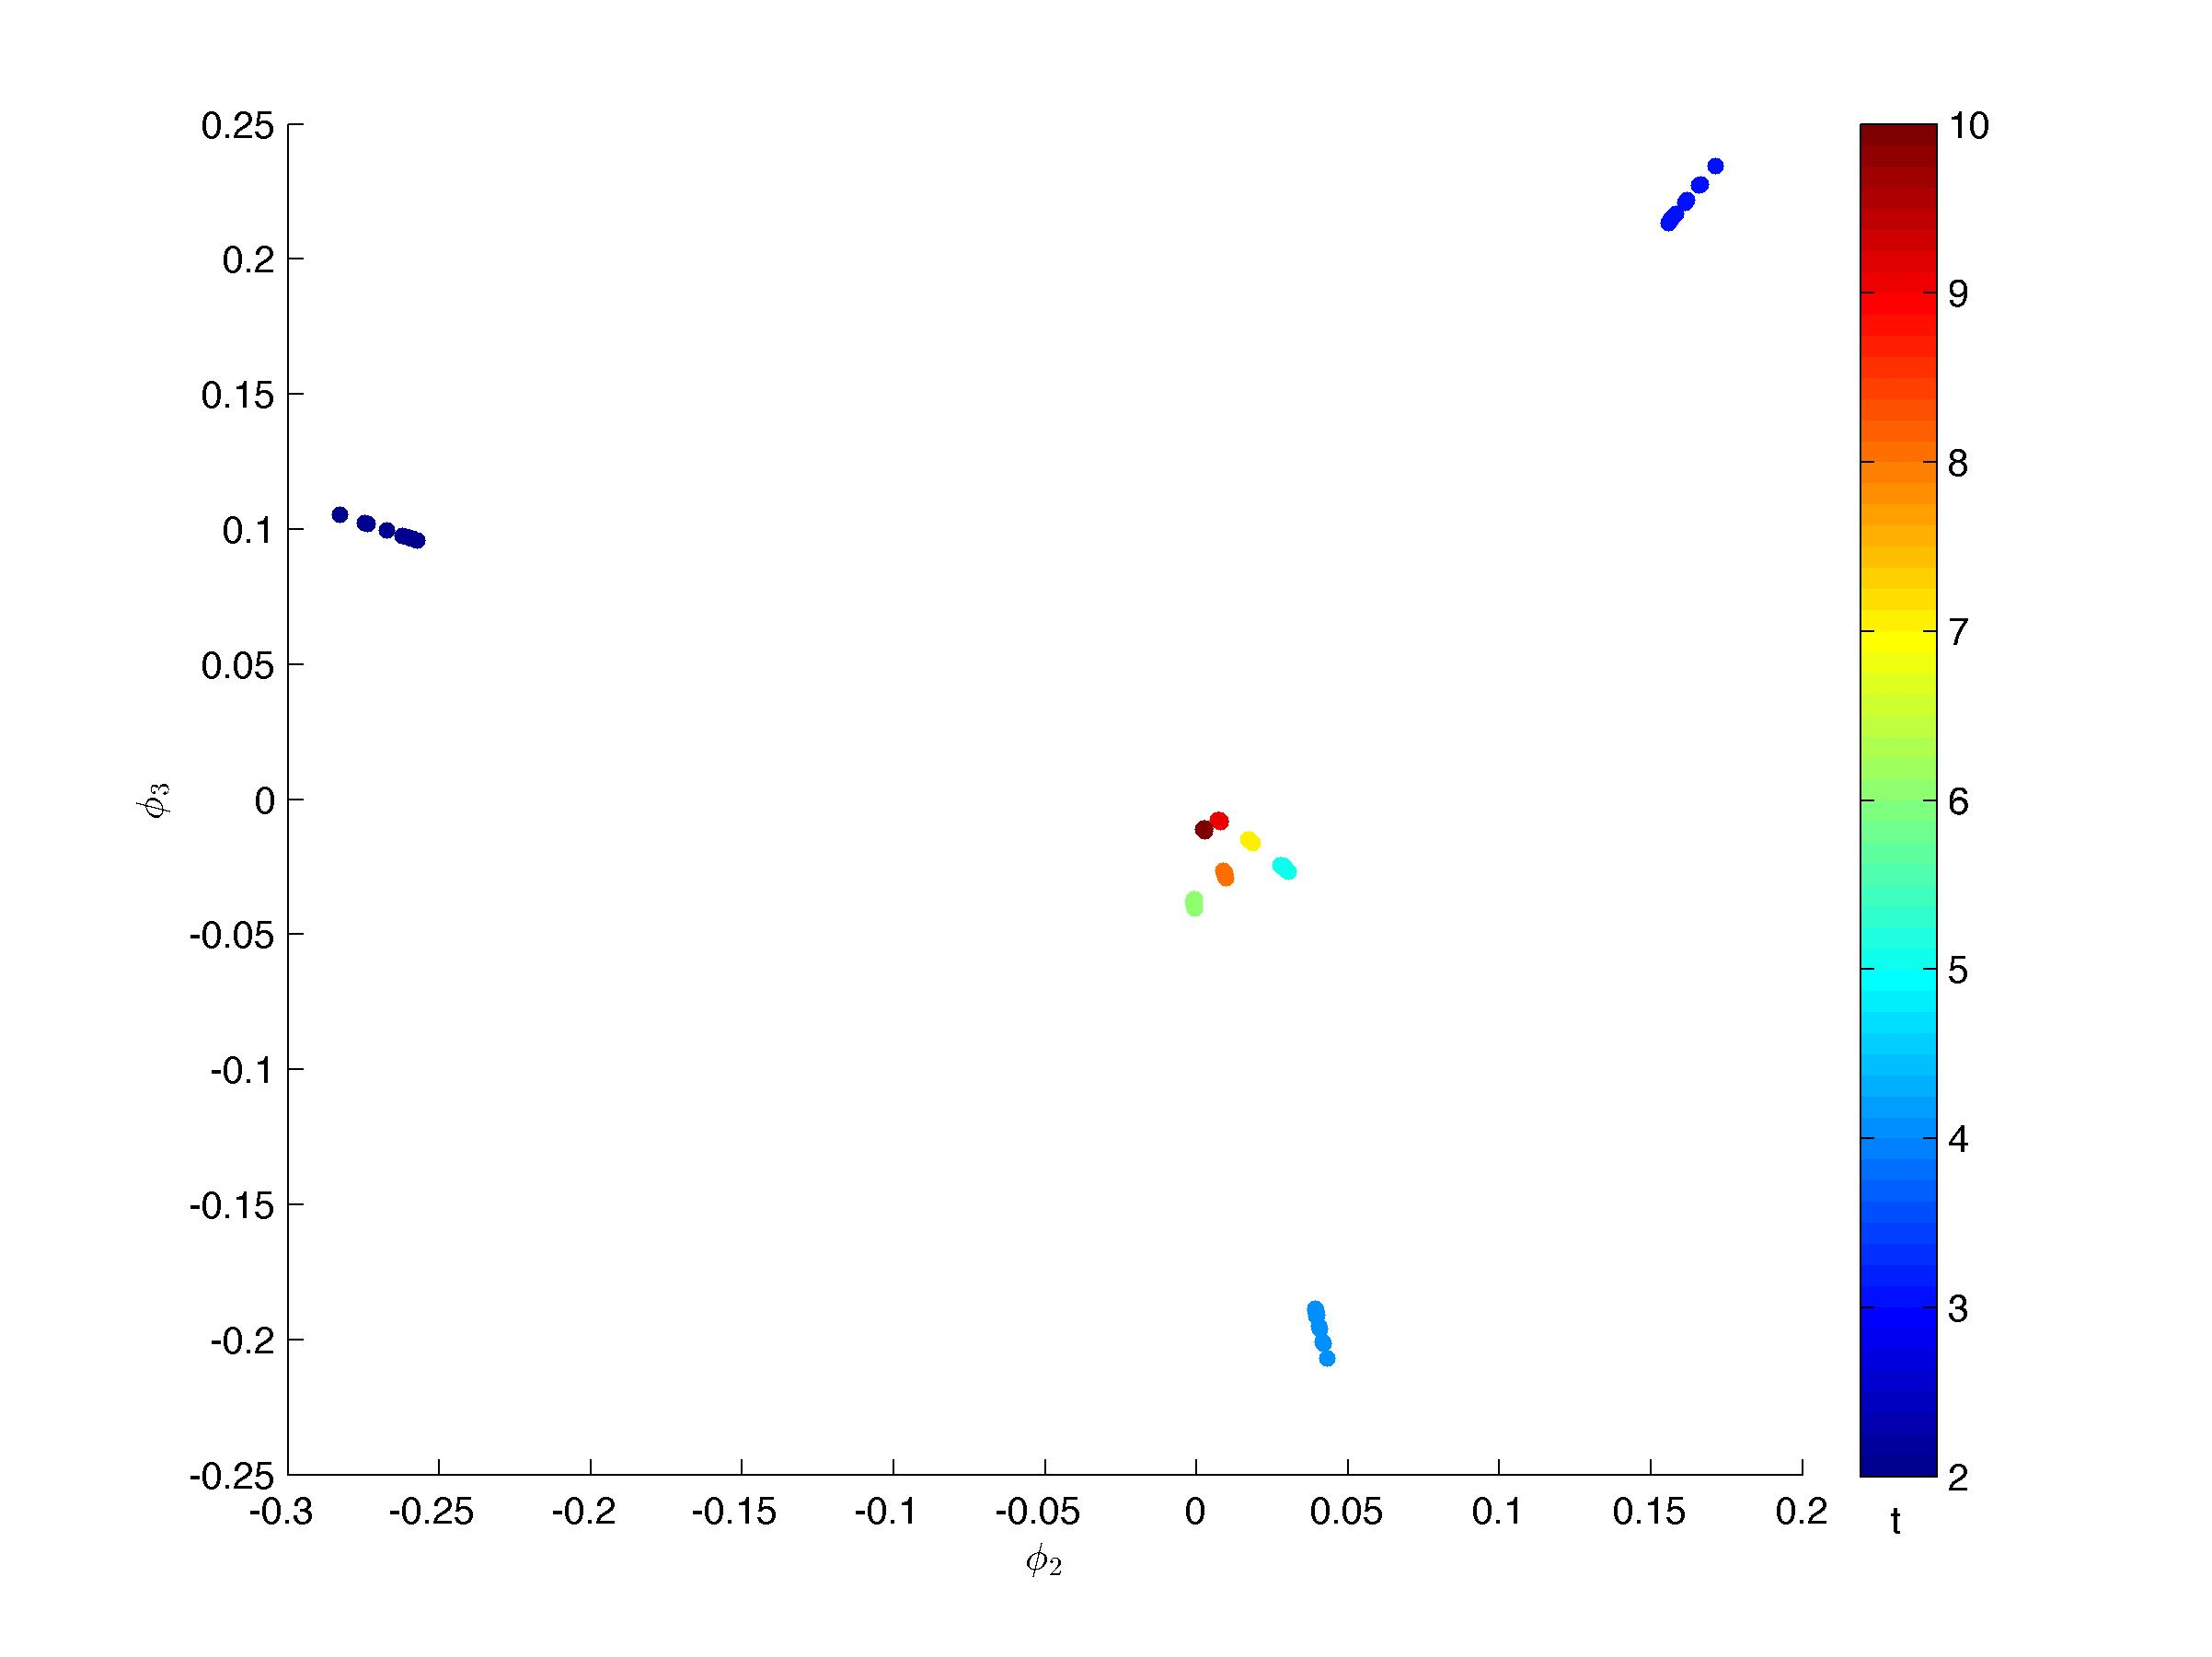
\includegraphics[width=\textwidth]{rawhist_t_1}
%%\caption{}
%%\end{subfigure}
%%\begin{subfigure}{\figwidth}
%%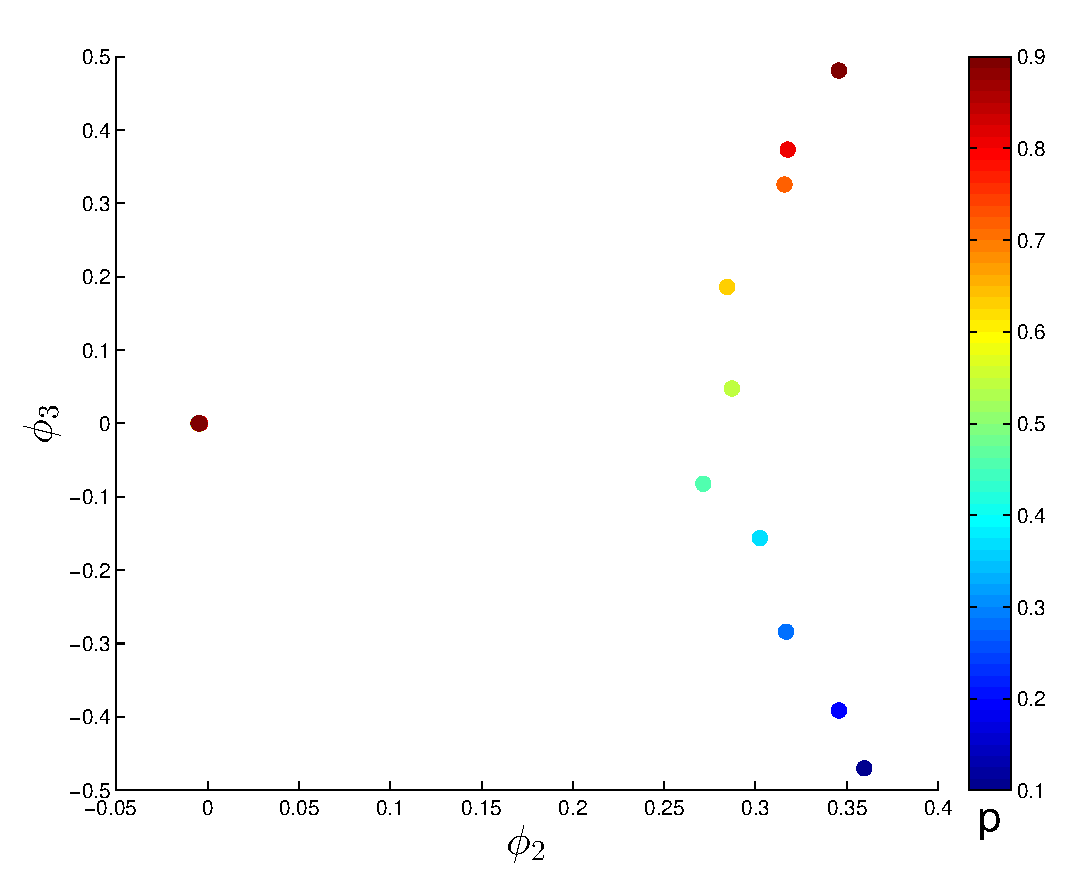
\includegraphics[width=\textwidth]{rawhist_p_400}
%%\caption{}
%%\end{subfigure}
%%\begin{subfigure}{\figwidth}
%%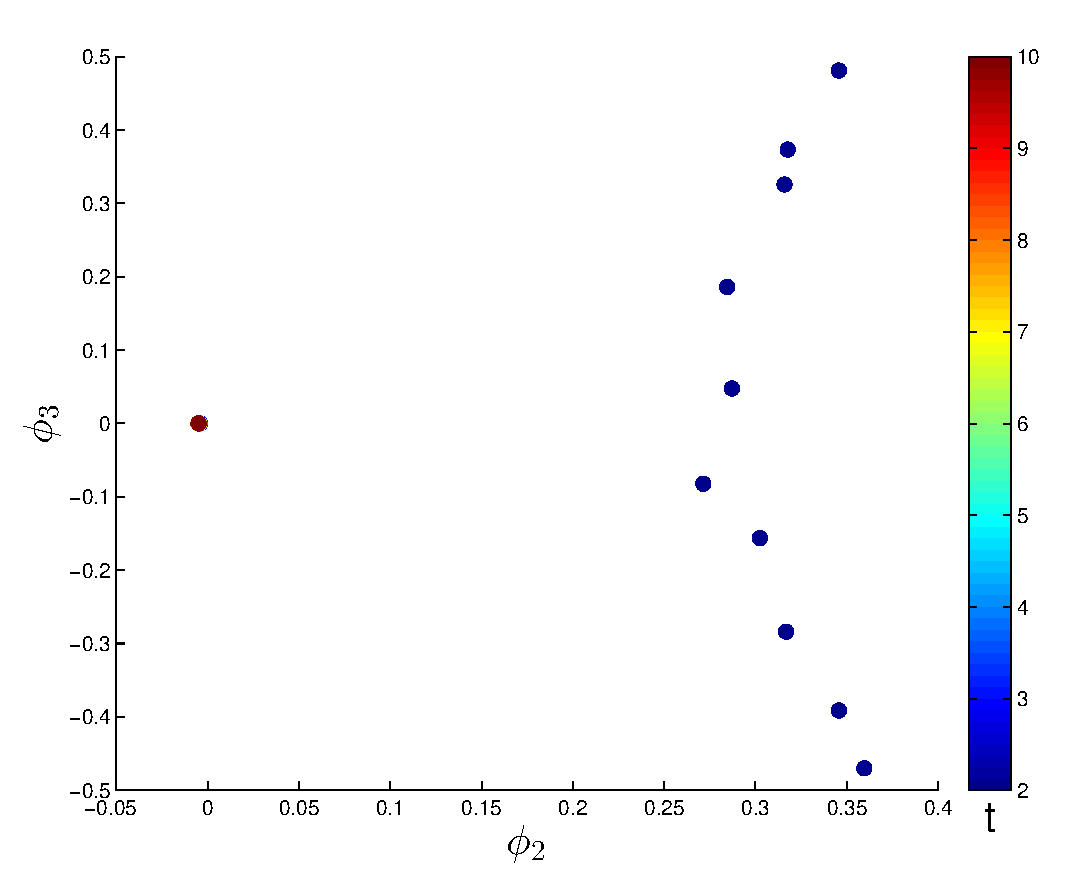
\includegraphics[width=\textwidth]{rawhist_t_400}
%%\caption{}
%%\end{subfigure}
%%\caption{Diffusion maps embeddings computed from simulation data of the velocity jump process with (a,b) $\lambda=1$, $s=1$, and (c,d) $\lambda=400$, $s=20$. The distances used in the diffusion maps kernel are the Euclidean distances between the histograms of particle positions. The data are colored by (a, c) $p$, the initial probability of a particle moving to the right, and (b, d) $t$, time.}
%%\label{fig:dmaps_embed_noemd}
%%\end{figure}




\subsubsection{Analytic macroscopic description}

This particular example has a known analytic macroscopic equation that governs the overall system behavior.
%
For a large collection of cells ($N \rightarrow \infty$), the system can be described by the probability density of the cells.
%
Let $\rho(x, t)$ denote the probability density of the cells, and let $\rho^-(x, t)$ and $\rho^+(x, t)$ denote the densities of the cells moving in the negative and positive axis directions, respectively.
%
It can be shown that, as $N \rightarrow \infty$, the densities satisfy the following set of partial differential equations (PDEs) \cite{othmer2000diffusion}:
\begin{equation} \label{eqn:coupled_pdes}
\begin{aligned}
\frac{\partial \rho^+}{\partial t} + s \frac{\partial \rho^+}{\partial x} & = -\lambda \rho^+ +\lambda \rho^- \\
\frac{\partial \rho^-}{\partial t} - s \frac{\partial \rho^-}{\partial x} & = \lambda \rho^+ -\lambda \rho^- 
\end{aligned}
\end{equation}
%
Alternatively, \eqref{eqn:coupled_pdes} can be rewritten as one, second--order PDE:
\begin{equation} \label{eq:second_order_pde}
\frac{\partial^2 \rho}{\partial t^2} + 2 \lambda \frac{\partial \rho}{\partial t} = s^2 \frac{\partial ^2 \rho}{\partial x^2}
\end{equation}
%
%We assume that $s^2/\lambda = D$ is constant, so that the dynamics of the probability density are governed by a {\em single} parameter $\lambda$.
%
From \eqref{eq:second_order_pde}, we see that, for fixed values of $\lambda$ and $s$, the macroscopic state of the system (the probability density of the cells) is indeed a function of two variables $p$ and $t$. 
%
This implies that for fixed $\lambda$ and $s$, the {\em microscopic} data in a high-dimensional ambient space (e.g., the positions of all $N$ cells) should lie on a two-dimensional manifold parameterized by $p$ and $t$, 
and uncovering the low-dimensional structure of the microscopic data reveals this manifold.
%
This is consistent with the results presented in Figures~\ref{fig:dmaps_embed_emd}~and~\ref{fig:chemotaxis_simulations_harmonics}, where the two-dimensional embeddings obtained from microscopic simulation data are one-to-one with $p$ and $t$.

We consider two asymptotic regimes of simulation.
%
When $\lambda \rightarrow 0$, the right-hand side of \eqref{eqn:coupled_pdes} tends to 0, and \eqref{eqn:coupled_pdes} becomes two uncoupled wave equations,
\begin{equation}
\begin{aligned}
\frac{\partial \rho^+}{\partial t} + s \frac{\partial \rho^+}{\partial x} & = 0 \\
\frac{\partial \rho^-}{\partial t} - s \frac{\partial \rho^-}{\partial x} & = 0.
\end{aligned}
\end{equation}
%alternatively, \eqref{eq:second_order_pde} becomes the second order wave equation,
%\begin{equation}
%\frac{\partial^2 \rho}{\partial t^2} = s^2 \frac{\partial ^2 \rho}{\partial x^2}.
%\end{equation}

%Dividing \eqref{eq:second_order_pde} by $\lambda > 0$ yields
%\[
%\frac{1}{\lambda} \frac{\partial^2 \rho}{\partial t^2} + 2 \frac{\partial \rho}{\partial t} = D \frac{\partial ^2 \rho}{\partial x^2}
%\]
When $\lambda \rightarrow \infty$, \eqref{eq:second_order_pde} approaches the heat equation,
\begin{equation}
2 \frac{\partial \rho}{\partial t} = D \frac{\partial ^2 \rho}{\partial x^2},
\end{equation}
%
where $D=s^2/\lambda$.
%
%Two variables determine the macroscopic state of the system: the initial distribution, which is controlled by a single parameter $p$, and the time, $t$.
%
The above analysis shows that the initial distribution of velocities of the particles (determined by $p$ in the microscopic simulations) plays a very different role depending on the value of $\lambda$.
%
When $\lambda \rightarrow 0$, the dynamics are described by two wave equations, and the initial distribution persists throughout the trajectory.
%
When $\lambda \rightarrow \infty$, the dynamics are described by one heat equation, and the initial conditions are insignificant -- the velocity distribution quickly equilibrates and we see purely diffusive behavior.
%

The relative importance of $p$ and $t$ from the analytic description are consistent with the results in Figure~\ref{fig:dmaps_embed_emd}, where $p$ appears as the ``more important'' coordinate when $\lambda$ is small and as the ``less important'' coordinate when $\lambda$ is large. 
%
Furthermore, in the small $\lambda$ regime (wave equation), shown in Figures \ref{subfig:small_lambda_p} and \ref{subfig:small_lambda_t}, the points corresponding to small times are more tightly clustered than the points corresponding to large times.
%
This is in agreement with the macroscopic model: at small times, the particles are more condensed around $x=0$, and it is more difficult to distinguish the particles moving to the left from the particles moving to the right. 
%
On the other hand, at large times, once the particles evolve from the origin, this separation is clear.  
%
For the large $\lambda$ case (heat equation), shown in Figures \ref{subfig:large_lambda_p} and \ref{subfig:large_lambda_t}, we observe that at small times, the initial distribution $p$ is well organized in the embedding in Figure \ref{subfig:large_lambda_p}, as the skew of the velocity distribution can be seen in the initial displacements.
%
On the other hand, for large times, we observe that the initial distribution $p$ is less organized in Figure \ref{subfig:large_lambda_p}, as the velocities have equilibrated and the initial distribution is less detectable in the particle density.
%
Overall, in both cases, we obtain, in an unsupervised data-driven manner, an accurate picture of the macroscopic variables that govern the system dynamics.


Furthermore, this analytic macroscopic descrption shows us that when $\lambda$ is small, the system dynamics can be described by the densities $\rho^+$ and $\rho^-$, and when $\lambda$ is large, the dynamics are described by $\rho = \rho^+ + \rho^-$. 
%
Figures~\ref{subfig:small_lambda_rho}~and~\ref{subfig:large_lambda_rho} show the data, colored by the difference in the average position of the left- and right-moving particles. 
%
Clearly, for small $\lambda$, where both $\rho^+$ and $\rho^-$ are required to describe the dynamics, the data is organized by the differences in the two densities. 
%
However, for large $\lambda$, the two densities rapidly equilibrate, and no organization based on the differences between the two densities is visible.  



%
%We will demonstrate how we can use diffusion maps to parameterize the simulation data, as well as detect the effective dimensionality of the data.
%
%We expect the simulation data to lie on a low-dimensional manifold which is parameterized by the macroscopic variables.
%
%We use diffusion maps \cite{coifman2005geometric}, which is a manifold learning technique, to uncover such low-dimensional structure and to analyze the results of the microscopic chemotaxis simulations.
%
%Compared to principal components analysis (PCA) \cite{shlens2005tutorial}, a standard linear technique, diffusion maps provides a parameterization of data which lie on a low-dimensional, (possibly) {\em nonlinear} structure in a high-dimensional space.
%
%Diffusion maps is one of many recently introduced manifold learning techniques that could be used to analyzed this data \cite{roweis2000nonlinear, tenenbaum2000global, Belkin2003}.



%correlations
%small lambda
%Euclidean: 3.3848e-04, -0.1861
%EMD: 0.9000, 0.9807
 %   
%large lambda
%Euclidean: -0.5466, 0.3329
%EMD: 0.9329, 0.9832

\subsubsection{Using an appropriate metric}

To emphasize the importance of using an appropriate distance metric, we analyzed the two sets of simulation data using the standard Euclidean distance between the histograms to compute the distances in \eqref{eq:W}.
%
We empirically found that there is no appreciable correlation between the embedding coordinates and the macroscopic variables $p$ and $t$ (the correlations between the embedding coordinates and the governing macroscopic variables are all  less than 60\%, with the correlations for the small $\lambda$ case being less than 20\%). 
%
In contrast, the correlations between the embedding coordinates and the macroscopic variables when using EMD in the diffusion maps calculation are all greater than 80\%.
%
This emphasizes the importance of using a metric which accurately describes the distances between observations.

\subsubsection{Detecting changes in dimensionality}

\begin{figure}[t]
%
\centering
\includegraphics[width=0.5\textwidth]{tmax_lambda_transition}
%
\caption{Detecting the change in dimensionality. The ratio of the log of the two eigenvalues which correspond to unique eigendirections is plotted as a function of the timescale of the simulation ($t_{max}$) and $\lambda$. Each data point is the average eigenvalue ratio over three data sets. Each data set consists of $10$ simulations, with initial conditions uniformly chosen such that $0.1 \le p  \le 0.9$. We allow each simulation to evolve for $t_{max}$ time units, with $dt=t_{max}/10$, and use data with $t > 0$ for analysis. The distances used in the diffusion maps kernel are the earth mover's distances between the histograms of particle positions. The curve $1/\lambda = t_{max}/N$ is shown in white. When the diffusive time scale is significantly larger than the drift time scale, the data is expected to be effectively one-dimensional. This transition is consistent with the empirical eigenvalues: the data are effectively one-dimensional when $t_{max}$ and/or $\lambda$ are large, since the first eigenvalue is significantly larger than the second. }
%
\label{fig:chemotaxis_compare_timescales_evals}
%
\end{figure}

Detecting changes in dimensionality is essential for the analysis and modeling of dynamical systems. 
%
For this example, we show that the true dimensionally of a data set can be estimated by looking at the eigenvalues corresponding to unique eigendirections. 
%
%For the specific chemotaxis example, we know that there are two directions in the data, corresponding to simulation parameters $p$ and $t$. 
%%
%However, for large values of $\lambda$, we know the dynamics become diffusive and $p$ becomes unimportant; we therefore expect the data to look approximately one-dimensional when $\lambda$ is large. 
%
%To detect this transition in the data, we look at the eigenvalues corresponding to the unique eigendirections. 
%
Let $\mu_{i_1} \ge \mu_{i_2}$ denote these two eigenvalues. 
%
According to \eqref{eq:est_lengths}, we plot  
\begin{equation}\label{eq:chemotaxis_eval_ratio}
 \sqrt{\frac{\log \mu_{i_1}}{\log \mu_{i_2}}} ;
\end{equation}
when this ratio becomes small, the data are effectively one-dimensional, as the second dimension is very small compared with the first. 
%



Figure~\ref{fig:chemotaxis_compare_timescales_evals} shows the eigenvalue ratio in \eqref{eq:chemotaxis_eval_ratio} as a function of $\lambda$ and the time scale of observation $t_{max}$, and we observe changes in the estimated dimensionality.
%
%We therefore expect the observed dimensionality to change from two to one as a function of $\lambda$. 
%
%For general dynamical systems, the governing macroscopic variables and asymptotic behavior may not be immediately obvious, and instead need to be inferred from the microscopic data.
%
For this specific example, these changes are consistent with the analytically-predicted shift when 
\begin{equation}
\frac{t_{max}}{N} = \frac{1}{\lambda}.
\end{equation} 
%
For small $\lambda$ and/or short $t_{max}$, the data are effectively two-dimensional, as both $p$ and $t$ are important to the observed dynamics. 
%
However, when $\lambda$ and/or $t_{max}$ is large, the system rapidly equilbrates and the data are effectively one-dimensional, parameterized by $t$. 
%
%From \cite{othmer2000diffusion}, the relevant time scales for the velocity jump process are
%%\begin{equation}
%%\begin{aligned}
%%\tau_{drift} =& \frac{L}{s} \\
%%\tau_{diff} =& \frac{L^2 \lambda}{s^2}
%%\end{aligned}
%%\end{equation}
%%%
%%Here, we take $L = t_{max} s$ as a characteristic length scale for the simulations. 
%%
%\begin{equation}
%\begin{aligned}
%\tau_{drift} =& t_{max} \\
%\tau_{diff} =& t_{max}^2 \lambda
%\end{aligned}
%\end{equation}
%%
%When $\frac{\tau_{diff}}{\tau_{drift}} =  t_{max}  \lambda \gg 1$, then the dynamics are effectively one-dimensional. 
%%
This ratio is also plotted in Figure~\ref{fig:chemotaxis_compare_timescales_evals} as a function of $\lambda$, and the transition is consistent with the transition predicted by the diffusion maps eigenvalues. 


\section{Conclusions}

This paper aims to bridge the fields of data mining and dynamical systems. 
%
For data mining methods to be informative with regards to the underlying system dynamics, processing the appropriate statistical moments or observables instead of individual particles is essential. 
%
In addition, one must also define the appropriate distance metric between the observations.
%
These two components induce the ``correct" Riemannian geometry and allow for informative analyses, such as meaningful and compact parameterization, phase shift detection, and dynamical characterization, through manifold learning.
%
In this paper, these concepts were demonstrated using a dynamical model of cellular chemotaxis with a known macroscopic behavior.
%
We showed that, using histograms as observers and EMD as a distance metric, diffusion maps can uncover a parameterization of the microscale data which is consistent with the analytic macroscopic model.
%
We are confident that such techniques can help inform modeling efforts for systems where the macroscopic dynamics and behavior are not currently known. 


\section*{Acknowledgment}
The authors would like to thank TODO.

\bibliographystyle{elsarticle-num}
\bibliography{../../../references/references}

\end{document}
